\documentclass[11pt]{article}

% Encoding and font handling
\usepackage[T1]{fontenc}
\usepackage[utf8]{inputenc}

% Math packages
\usepackage{amsmath, amssymb, amsthm}
\newtheorem{proposition}{Proposition}
\newcommand{\softmax}{\mathrm{softmax}}
\newcommand{\TopK}{\operatorname{TopK}}

% Graphics, floats, and layout
\usepackage{graphicx}
\usepackage[font=small,labelfont=bf]{caption}
\usepackage{float}
\usepackage[margin=1in]{geometry}
\usepackage[protrusion=true, expansion=false]{microtype}

% Algorithms and tables
\usepackage{algorithm}
\usepackage{algorithmic}
\usepackage{booktabs, enumitem}

% Bibliography
\usepackage[backend=biber, style=numeric, sorting=none]{biblatex}
\addbibresource{references.bib}

% Hyperlinks and clever references
\usepackage[colorlinks=true, linkcolor=blue, urlcolor=blue, citecolor=blue]{hyperref}
\usepackage{cleveref}

% Header and footer customization
\usepackage{fancyhdr}
\pagestyle{fancy}
\fancyhf{}
\fancyhead[L]{\textsc{X-Spanformer}}
\fancyhead[R]{\textsc{Span-Aware Encoder}}
\fancyfoot[C]{\thepage}
\setlength{\headheight}{14pt}

% Document spacing and typography
\setlength{\parindent}{0pt}
\setlength{\parskip}{6pt}
\setlength{\emergencystretch}{3em}
\addtolength{\topmargin}{-2pt}
\sloppy

% Metadata
\title{\textbf{X-Spanformer: A Tokenizer-Free, Span-Aware Encoder Inspired by X-Bar Theory}}
\author{
	Kara Marie Rawson\thanks{\href{mailto:rawsonkara@gmail.com}{rawsonkara@gmail.com}} \and
	Aimee Chrzanowski\thanks{\href{mailto:aimeechrzanowski@gmail.com}{aimeechrzanowski@gmail.com}}
}
\date{\today}

\begin{document}
	
	% Cover image
	\begin{figure}[H]
		\centering
		
\includegraphics[width=0.95\textwidth]{figures/figure_00.png}
	\end{figure}
	\vspace{2em}
	
	\maketitle
	
	\begin{center}
		\textit{This work is a preprint and has not yet been peer reviewed.}
	\end{center}
	
	% Section includes
	\begin{abstract}
	Tokenization remains a fundamental bottleneck in transformer architectures, as static subword vocabularies fragment cross-domain text and impede real-time adaptability. We introduce X-Spanformer, a tokenizer-free, span-aware segmentation front end inspired by X-bar theory. X-Spanformer begins by inducing a hybrid Unigram-LM vocabulary—comprising all UTF-8 codepoints plus top entropy-pruned subword fragments—via an EM procedure approximated with Viterbi decoding, then applies a learned pruning criterion based on per-piece perplexity and OOV rate; this entire process is implemented as an efficient ONNX custom operator. The resulting soft piece-assignment matrix \(P\in\mathbb{R}^{T\times V}\) is embedded and contextualized through a lightweight convolutional encoder that scales linearly in \(T\). A factorized pointer network then identifies overlapping, variable-length spans, which are softly typed by modality, filtered by a learned length estimator, and pooled into \(d\)-dimensional span embeddings. We retain the top-\(K\) spans and fuse them via relevance-weighted interpolation into a single controller vector \(s\), which is injected into downstream transformer layers through prefix-token, attention-bias, or gated fusion pathways. X-Spanformer is trained with an entropy-regularized span induction curriculum transitioning from synthetic supervision to type-aware signals. Empirical evaluation on compression ratio, contrastive retrieval alignment, span entropy, modality coherence, and end-to-end inference speed demonstrates that X-Spanformer outperforms static BPE and byte-level baselines in structural interpretability, compression efficiency, and throughput. An open-source ONNX-compatible implementation, along with training recipes and corpus construction guidelines, is provided to facilitate adoption across code, language, and hybrid domains.
\end{abstract}

	\section{Introduction}

Transformer architectures have become the foundation for advances in natural language understanding, program synthesis, and multimodal retrieval \cite{vaswani2017attention,devlin2019bert,radford2019gpt2,raffel2020t5}.  A critical precondition for these models is the segmentation of raw text into discrete units—most commonly fixed subwords produced by Byte‐Pair Encoding (BPE) \cite{sennrich2016bpe} or SentencePiece \cite{kudo2018sentencepiece}.  While such static vocabularies yield efficient lookup and in‐domain accuracy, they impose irrevocable lexical boundaries that (i) degrade under domain shift \cite{galle2021respite}, (ii) obscure long‐range compositional patterns in code and multilingual text, and (iii) demand costly re‐training or vocabulary expansion to accommodate novel syntax or semantics.

Segmentation is traditionally decoupled from model training, treated as an irreversible preprocessing step that precludes gradient flow and adaptation to downstream objectives.  Recent work in character‐aware encoding and tokenization‐free models—such as Charformer \cite{tay2021charformer}, CANINE \cite{clark2021canine}, and probabilistically masked language models \cite{liu2022learnedsegmentation,liu2022pmlm}—demonstrates the potential of integrating segmentation into end‐to‐end learning.  However, these methods either omit explicit linguistic priors or fail to produce interpretable, overlapping segments aligned with phrase‐level semantics.

Drawing on the X‐bar schema from generative grammar \cite{jackendoff1977xbar}, we introduce X-Spanformer, a span‐based segmentation module that is fully differentiable and ONNX‐native.  X-Spanformer begins with a hybrid Unigram‐LM front‐end—combining all UTF-8 characters with top entropy‐pruned subword fragments via SentencePiece’s Unigram mode—to compute a soft probability matrix \(P\in\mathbb{R}^{T\times V}\) over raw Unicode codepoints.  A factorized pointer network \cite{vinyals2015pointer} then predicts variable‐length, overlapping span candidates, which are softly typed by modality, filtered by a learned length estimator, and pooled into \(d\)‐dimensional embeddings.  These embeddings are fused into a single controller vector \(s\) via relevance‐weighted interpolation and injected into downstream transformers through prefix, attention‐bias, or gated‐FFN pathways.  Because all components are differentiable, X-Spanformer supports end‐to‐end optimization of segmentation and task objectives, while maintaining compressor efficiency and interpretability.

\subsection{Contributions}

This paper makes the following contributions:
\begin{enumerate}
	\item We formalize tokenizer‐free segmentation as a span‐prediction problem grounded in X‐bar theory, instantiated with a hybrid Unigram‐LM front‐end, dynamic span capping, and modality typing.
	\item We propose a multi‐phase curriculum that bootstraps span induction from synthetic BPE labels and transitions to entropy‐regularized and type‐aware supervision.
	\item We design an ONNX‐native architecture for compositional pooling and controller fusion, detailing prefix‐token, attention‐bias, and gated‐FFN injection modes.
	\item We introduce an evaluation framework—covering compression ratio, contrastive retrieval alignment, span entropy, and modality coherence—and release an ONNX‐compatible implementation with training recipes and corpus construction guidelines.
\end{enumerate}
	\section{Related Work}

\subsection{Static Subword Tokenization}
Conventional transformer pipelines rely on fixed subword vocabularies, most prominently Byte‐Pair Encoding (BPE) \cite{sennrich2016bpe} and Unigram‐LM tokenizers such as SentencePiece \cite{kudo2018sentencepiece}. These methods facilitate efficient embedding lookup and strong in‐domain performance, but their immutable vocabularies cannot adapt during training, fragment compositional or rare phrases under domain shift \cite{galle2021respite}, and necessitate costly re‐tokenization when new syntax or terminology arise.

\subsection{Character- and Byte-Level Encoders}
To eliminate subword heuristics, character‐ and byte‐level models process raw codepoints directly. Charformer \cite{tay2021charformer} learns latent splits via gradient‐based tokenization, CANINE \cite{clark2021canine} applies down‐ and up‐sampling around raw Unicode, and ByT5 \cite{xue2022byt5} explores purely byte‐level inputs. While these approaches remove offline segmentation, they do not produce overlapping or hierarchical spans and rely on global self‐attention for context.

\subsection{Differentiable Segmentation}
Unsupervised and differentiable segmentation integrates boundary induction into neural pretraining. Morfessor \cite{creutz2005unsupervised} applies minimum description‐length to discover morphemes. Probabilistically Masked Language Models \cite{liu2022pmlm} and learned‐segmentation models \cite{liu2022learnedsegmentation} optimize reconstruction objectives to induce non‐overlapping partitions. These methods enable end‐to‐end learning but lack explicit modeling of overlapping spans or linguistic structure.

\subsection{Span-Based and Pointer Networks}
Pointer networks \cite{vinyals2015pointer} predict arbitrary start–end pairs to locate variable‐length spans. SpanBERT \cite{joshi2020spanbert} leverages this for masked span reconstruction, and similar architectures in vision and speech generate overlapping proposals for improved alignment \cite{ren2015faster,zach2019segmenter}. However, prior work has not combined pointer‐based, overlapping span induction with explicit grammar‐inspired priors within transformer encoders.

\subsection{Bridging Static and Dynamic Segmentation}
Hybrid vocabularies that merge character coverage with static subwords have been proposed to improve robustness \cite{tay2021charformer,clark2021canine}. Our approach extends this paradigm by training a hybrid Unigram‐LM front end—induced by an EM procedure approximated via Viterbi decoding and pruned on perplexity and OOV thresholds—implemented as an ONNX custom operator. We then employ a convolutional encoder to contextualize soft assignments, a factorized pointer network to propose overlapping spans, and a modality‐aware scoring mechanism to filter and fuse spans into a controller vector for downstream transformer injection.

\medskip
In contrast to purely static tokenizers, character‐level models, and non‐overlapping segmentation methods, X‐Spanformer unifies hybrid vocabulary induction, differentiable Viterbi‐based pruning, convolutional contextualization, and pointer‐network span prediction under a single, ONNX‐native framework. This design yields dynamic, interpretable spans that adapt to domain shifts and can be optimized end‐to‐end alongside downstream tasks.  
	\section{Architecture}

This section formalizes the modular components of X-Spanformer and their interactions within the segmentation pipeline.  Each architectural unit is motivated, given a precise mathematical formulation, and illustrated with pseudocode where appropriate.  We conclude with strategies for integrating the fused span controller into standard transformer encoders and analyze runtime complexity.

X-Spanformer begins with a hybrid Unigram-LM vocabulary\footnote{Learned via EM over substrings up to length \(L_{\max}\); see Sec.~\ref{sec:vocab-induction} for details.} that replaces hard token boundaries with soft, probabilistic segmentation.  A custom ONNX operator ingests raw Unicode codepoints of length \(T\) and computes a probability matrix  
\[
P \;\in\;\mathbb{R}^{T\times V}, 
\quad
P_{t,i} = \Pr(\text{piece }u_i\text{ starts at position }t),
\]
where \(V\) is the induced vocabulary size.  We embed these soft piece probabilities via  
\[
H^0 = P\,W_{\mathrm{emb}},
\quad
W_{\mathrm{emb}}\in\mathbb{R}^{V\times d},
\]
yielding seed embeddings \(H^0\in\mathbb{R}^{T\times d}\).  From these low-level vectors, the model:

\begin{itemize}
	\item Extracts a ranked span set \(S=\{(i_k,j_k)\}_{k=1}^K\) with \(1\le i_k<j_k\le T\) via a pointer network \cite{vinyals2015pointer}.
	\item Pools each span \((i_k,j_k)\) into a \(d\)-dimensional embedding \(s_{i_kj_k}\) (mean or gated pooling) \cite{tay2021charformer}.
	\item Predicts soft modality distributions \(p^\mathrm{type}_{i_kj_k}\in\Delta^M\), reflecting types such as code, natural language, or identifier \cite{lin2021codemix,li2021prefix}.
	\item Filters down to a final span set \(S'\subseteq S\) via a learned length estimator \cite{cheng2021masked}.
\end{itemize}

Span-level augmentation parallels auxiliary token insertion in models like SpanBERT \cite{joshi2020spanbert} but operates on soft, overlapping spans rather than hard subwords.  All modules—from boundary scoring to controller fusion—are fully differentiable and trained end-to-end with the downstream encoder.

% New subsection: vocabulary induction
\subsubsection{Dataset Extraction and Validation}
\label{sec:dataset-extraction}

Our segmentation pipeline begins by converting raw PDF documents into judged text segments.  We first apply the \texttt{pdf2seg} tool, which performs layout-aware OCR to extract candidate snippets.  Each CSV record includes the Unicode codepoint sequence, bounding-box metadata, and an OCR confidence score.  Records failing heuristic filters—such as non-text artifacts, control-character noise, or confidence below a threshold—are flagged and excluded.

Validated CSV records are then ingested by \texttt{pdf2jsonl}, which normalizes Unicode, merges overlapping snippets, and emits a clean JSONL dataset.  During this conversion we remove duplicates, discard empty segments, and log all excluded records for audit.  The resulting corpus of high-quality, human-judged text segments serves as the input to our vocabulary induction and span modeling stages.

We considered augmenting each validated segment with multiple paraphrases (e.g., three per segment) to increase diversity, but this introduces substantial preprocessing overhead and can distort structural cues.  Instead, we expand corpus coverage by ingesting additional PDFs, ensuring scale and domain variety without paraphrase-induced noise.
\subsection{Hybrid Unigram‐LM Vocabulary Induction}
\label{sec:vocab-induction}

We construct a data‐adaptive subword vocabulary by training a Unigram language model (LM) over all substrings up to length \(L_{\max}\), then pruning pieces based on both corpus perplexity and coverage (OOV rate). Let
\(\mathcal X = \{x^{(i)}\}_{i=1}^N\)
be our corpus of raw Unicode codepoint sequences of total length \(T\), and let \(\mathcal U_{0}\) denote the initial candidate set formed by extracting every substring of length \(\le L_{\max}\), retaining the top \(M\) by frequency, and including all individual codepoints.

\subsubsection{Candidate Generation}

For each sequence \(x \in \mathcal X\), we slide a window of width \(\le L_{\max}\) across all codepoints to extract substrings. We record their frequency and retain the top \(M\) most frequent substrings. The resulting candidate set is:
\[
\mathcal U_{0}
= \{\text{top }M\text{ substrings}\} \cup \{\text{all single codepoints}\},
\]
ensuring base coverage and bounding vocabulary size.

\subsubsection{Unigram LM via EM}

We initialize the piece probabilities by normalizing raw frequency counts:
\[
p^{(0)}(u)
= \frac{\mathrm{freq}(u)}{\sum_{v\in\mathcal U_{0}}\mathrm{freq}(v)},
\quad
\forall\,u\in\mathcal U_{0}.
\]

At each EM iteration \(t\), we alternate:

\paragraph{E-step:}

For each sequence \(x\in\mathcal X\), we compute the posterior usage mass \(\gamma^{(t)}(u \mid x)\) for every piece \(u\in \mathcal U_t\). Since enumerating all segmentations of \(x\) is intractable, we approximate using the single best segmentation:
\[
\mathrm{seg}^{*}(x)
= \arg\max_{\mathrm{seg}} \prod_{v\in\mathrm{seg}} p^{(t)}(v),
\]
obtained via Viterbi decoding \cite{kudo2018sentencepiece}. We then compute:
\[
\gamma^{(t)}(u \mid x)
= \sum_{v \in \mathrm{seg}^{*}(x)} \mathbf{1}_{u = v}.
\]

\paragraph{M-step:}

We re-estimate the piece probabilities as:
\[
p^{(t+1)}(u)
= \frac{
	\sum_{x \in \mathcal X} \gamma^{(t)}(u \mid x)
}{
	\sum_{v \in \mathcal U_t} \sum_{x \in \mathcal X} \gamma^{(t)}(v \mid x)
},
\]
which reduces to relative frequency over the Viterbi segmentations.

\subsubsection{Baseline Perplexity}

To benchmark compressibility before pruning, we compute the initial corpus perplexity:
\[
\mathrm{PPL}^{(0)}
= \exp\left(
-\frac{1}{|\mathcal X|} \sum_{x\in\mathcal X} \log \prod_{v \in \mathrm{seg}^{*}(x)} p^{(0)}(v)
\right),
\]
where \(\mathrm{seg}^{*}(x)\) is the Viterbi segmentation under \(p^{(0)}\).







\subsubsection{Adaptive Pruning by PPL and OOV}

After each M‐step, we consider pruning any piece \(u\in V\) with \(p^{(t)}(u)<\epsilon\).  For a candidate removal \(V' = V \setminus \{u\}\), we first perform Viterbi segmentation under the reduced vocabulary:

\[
\mathrm{seg}^{*}_{V'}(x) \;=\;\arg\max_{\mathrm{seg}} \;\prod_{v\in\mathrm{seg}} p^{(t)}_{V'}(v)
\quad\text{for each }x\in\mathcal X.
\]

We then introduce the following quantities:

\[
N_{p}' \;=\;\sum_{x\in\mathcal X} \bigl|\mathrm{seg}^{*}_{V'}(x)\bigr|
\quad\text{(total number of subword pieces)},
\]

\[
L' \;=\; -\,\sum_{x\in\mathcal X}\;\sum_{v\in\mathrm{seg}^{*}_{V'}(x)}\log p^{(t)}_{V'}(v)
\quad\text{(negative log‐likelihood of all pieces)},
\]

\[
N_{t} \;=\;\sum_{x\in\mathcal X} |x|
\quad\text{(total number of codepoint tokens)},
\]

\[
N_{\mathrm{uncov}}' 
\;=\; \sum_{x\in\mathcal X}\;\sum_{i=1}^{|x|}
\mathbf1\bigl(i\not\in \mathrm{cover}_{V'}(x)\bigr)
\quad\text{(total uncovered positions)},
\]

where \(\mathrm{cover}_{V'}(x)\) is the set of codepoint indices spanned by \(\mathrm{seg}^{*}_{V'}(x)\).

Using these, we define:

\[
\mathrm{PPL}' 
= \exp\Bigl(\tfrac{L'}{N_{p}'}\Bigr),
\quad
\mathrm{OOV}' 
= \frac{N_{\mathrm{uncov}}'}{N_{t}}.
\]

We accept the removal \(u\) if and only if both
\[
\mathrm{PPL}' - \mathrm{PPL}^{(t)} < \tau_{\mathrm{ppl}}
\quad\text{and}\quad
\mathrm{OOV}' \le \delta_{\mathrm{oov}}.
\]

This criterion guarantees that any pruning step degrades the model’s average piece‐level log‐likelihood by at most \(\tau_{\mathrm{ppl}}\) and introduces no more than \(\delta_{\mathrm{oov}}\) uncovered codepoint positions.









\subsubsection{Existence and Monotonicity Proposition}

Define the feasible set:
\[
\mathcal F(\tau,\delta)
= \left\{\,V\subseteq\mathcal U_{0}\,\middle|\,
\mathrm{PPL}(V)\le \mathrm{PPL}^{(0)}+\tau,\;
\mathrm{OOV}(V)\le \delta
\right\}.
\]

\begin{proposition}[Feasibility and Monotonicity]
	For any \(\tau,\delta \ge 0\), the feasible set \(\mathcal F(\tau,\delta)\) is nonempty. Moreover, if \(\tau' \ge \tau\), \(\delta' \ge \delta\), then:
	\[
	\mathcal F(\tau,\delta) \subseteq \mathcal F(\tau',\delta'),
	\quad
	\Rightarrow
	\quad
	\min_{V\in\mathcal F(\tau',\delta')}|V| \le \min_{V\in\mathcal F(\tau,\delta)}|V|.
	\]
\end{proposition}

\begin{proof}
	\textbf{Step 1: Existence}
	
	Choose \(V = \mathcal U_0\), the full candidate set.
	
	Since \(V\) includes all substrings and individual codepoints:
	\[
	\mathrm{OOV}(V) = 0,
	\quad
	\mathrm{PPL}(V) = \mathrm{PPL}^{(0)}.
	\]
	
	Therefore, for any \(\tau,\delta \ge 0\),
	\[
	\mathrm{PPL}(V) \le \mathrm{PPL}^{(0)} + \tau,
	\quad
	\mathrm{OOV}(V) \le \delta,
	\quad
	\Rightarrow
	V \in \mathcal F(\tau,\delta).
	\]
	
	\textbf{Step 2: Monotonicity}
	
	Let \(V \in \mathcal F(\tau,\delta)\), and suppose \(\tau' \ge \tau\), \(\delta' \ge \delta\). Then:
	\[
	\mathrm{PPL}(V) \le \mathrm{PPL}^{(0)} + \tau \le \mathrm{PPL}^{(0)} + \tau',
	\quad
	\mathrm{OOV}(V) \le \delta \le \delta',
	\quad
	\Rightarrow
	V \in \mathcal F(\tau',\delta').
	\]
	
	Thus:
	\[
	\mathcal F(\tau,\delta) \subseteq \mathcal F(\tau',\delta').
	\]
	
	\textbf{Step 3: Minimality}
	
	Since \(\mathcal F(\tau,\delta) \subseteq \mathcal F(\tau',\delta')\),
	\[
	\min_{V \in \mathcal F(\tau',\delta')} |V| \le \min_{V \in \mathcal F(\tau,\delta)} |V|.
	\]
\end{proof}

\subsubsection{Algorithm: Adaptive Vocabulary Induction}

To construct an efficient and corpus-aware subword vocabulary, we apply an expectation-maximization loop over the candidate set \(\mathcal{U}_0\), guided by a Viterbi-decoded likelihood objective. Starting from raw frequency estimates, we refine piece probabilities \(p(u)\) via best-segmentation token counts and normalize them across the corpus. After each M-step, we attempt to prune low-probability pieces while preserving compressibility and coverage. Each candidate removal is simulated by resegmenting \(\mathcal{X}\) under the reduced vocabulary \(V'\) and evaluating both perplexity and position-level OOV rate. If the degradation in log-likelihood is bounded and no coverage gaps are introduced, the removal is accepted. This selective pruning yields a compact, entropy-regularized vocabulary tailored to the domain structure.

\begin{algorithm}[H]
	\caption{Adaptive Unigram‐LM Vocabulary Induction}
	\label{alg:vocab-induction}
	\begin{algorithmic}[1]
		\STATE Extract candidate substrings up to length \(L_{\max}\) from corpus \(\mathcal{X}\); form initial vocabulary \(\mathcal{U}_0\)
		\STATE Initialize piece probabilities: \(p^{(0)}(u) \propto \mathrm{freq}(u)\) for all \(u \in \mathcal{U}_0\)
		\STATE Compute baseline perplexity \(\mathrm{PPL}^{(0)}\) via Viterbi decoding over \(\mathcal{X}\)
		\FOR{iteration \(t = 0\) to \(T_{\max}\)}
		\FOR{each sequence \(x \in \mathcal{X}\)}
		\STATE Compute best segmentation \(\mathrm{seg}^{*}(x)\) using current \(p^{(t)}\)
		\STATE Accumulate token usage counts \(\gamma^{(t)}(u \mid x)\) for all \(u \in \mathrm{seg}^{*}(x)\)
		\ENDFOR
		\STATE Update probabilities: normalize counts to get \(p^{(t+1)}(u)\)
		\STATE Set current vocabulary \(V = \{u \mid p^{(t+1)}(u) > 0\}\)
		\FOR{each \(u \in V\) with \(p^{(t+1)}(u) < \epsilon\)}
		\STATE Tentatively prune: define \(V' = V \setminus \{u\}\)
		\FOR{each sequence \(x \in \mathcal{X}\)}
		\STATE Decode \(\mathrm{seg}^{*}_{V'}(x)\) using updated \(V'\)
		\STATE Compute log-prob score and uncovered positions
		\ENDFOR
		\STATE Compute \(\mathrm{PPL}'\) and \(\mathrm{OOV}'\) from new segmentations
		\IF{\(\mathrm{PPL}' - \mathrm{PPL}^{(t)} < \tau_{\mathrm{ppl}}\) and \(\mathrm{OOV}' \le \delta_{\mathrm{oov}}\)}
		\STATE Accept removal: \(V \leftarrow V'\)
		\ENDIF
		\ENDFOR
		\STATE Update \(\mathrm{PPL}^{(t+1)}\) using accepted vocabulary \(V\)
		\ENDFOR
		\STATE \textbf{Return} final pruned vocabulary \(V\) and piece probabilities \(\{p(u)\}\)
	\end{algorithmic}
\end{algorithm}
\subsection{Seed Embeddings and Candidate Set}
\label{sec:seed-embeddings}

The X-Spanformer pipeline begins with a sequence of \(T\) raw Unicode codepoints. We apply our custom Unigram‐LM operator (Sec.~\ref{sec:vocab-induction}), implemented as an ONNX custom op, to compute soft piece probabilities over the induced vocabulary \(V\):
\[
P \;\in\;\mathbb{R}^{T\times V},
\quad
P_{t,i} = \Pr\bigl(\text{piece }u_i\text{ starts at position }t\bigr).
\]
The vocabulary \(V\) comprises all single codepoints plus the final entropy‐ and perplexity‐pruned subword fragments.

These probabilities are embedded via a single matrix multiplication:
\[
H^0 = P\,W_{\mathrm{emb}},
\quad
W_{\mathrm{emb}}\in\mathbb{R}^{V\times d},
\]
yielding initial seed embeddings \(H^0\in\mathbb{R}^{T\times d}\) for each input position.

\subsubsection{Contextual Encoder: Convolutional Pathway}

To enrich these seed embeddings with contextual structure, we apply a lightweight convolutional encoder\footnote{We use dilated 1D convolutions with kernel sizes [3, 5, 7] and dilation rates [1, 2, 4] to capture multi-scale local patterns without quadratic complexity.} to produce the final representation \(H\in\mathbb{R}^{T\times d}\):
\[
H = \mathrm{ConvNet}(H^0),\quad \text{cost }O(T d^2).
\]
This encoder employs stacked or dilated 1D convolutions \cite{tay2021charformer}, providing fixed-window receptive fields that are tuned to capture short-range compositional patterns. By avoiding the quadratic complexity of self-attention, the convolutional encoder ensures scalability across long codepoint sequences and maintains a runtime that is linear in the input length.

The design choice to adopt convolutional contextualization reflects the architectural goal of high-throughput segmentation in real-time or resource-constrained settings. While transformer-based encoders offer richer modeling of long-distance dependencies \cite{vaswani2017attention}, their runtime limits applicability for streaming inputs or modular deployments. In contrast, convolutional filters preserve local positional regularities critical for span induction—such as those arising in identifiers, literals, or markup—and enable reproducible, interpretable segmentation across diverse modalities. Empirical evidence on synthetic benchmarks further suggests that this encoder achieves robust span localization without sacrificing structural fidelity \cite{rawson2025streammix}.

\subsubsection{Span Candidate Enumeration}

Given the contextualized sequence \(H\), we enumerate all contiguous span candidates:
\[
C = \{(i,j)\mid 1 \le i < j \le T,\quad j - i + 1 \le w_{\max}\}.
\]
This restricts span width to \(w_{\max}\), reducing total candidates from quadratic to linear scale: \(|C| = O(T\,w_{\max})\). Each span \((i,j)\) corresponds to the subsequence \([h_i,\dots,h_j]\), which is passed to the boundary scorer and length filter in subsequent modules. The candidate set remains compatible with global-attention filtering and sparse attention schemes \cite{joshi2020spanbert,tay2021charformer}, ensuring scalability and modularity in downstream processing.
\subsection{Span Predictor}
\label{sec:span-predictor}

Given contextualized embeddings 
\[
H \;\in\;\mathbb{R}^{T\times d},
\]
we first form the candidate span set:
\[
C \;=\;\{(i,j)\mid 1 \le i < j \le T,\; j - i \le w_{\max}\},
\]
as defined in Sec.~\ref{sec:seed-embeddings}. We then use two parallel linear heads—forming a factorized pointer network \cite{vinyals2015pointer}—to predict span boundaries:
\[
\ell^s = W_s\,H + b_s,
\quad
p^s = \softmax(\ell^s),
\qquad
\ell^e = W_e\,H + b_e,
\quad
p^e = \softmax(\ell^e),
\]
where \(W_s,W_e\in\mathbb{R}^{T\times d}\), \(b_s,b_e\in\mathbb{R}^T\), and \(p^s_i\), \(p^e_j\) denote the probabilities that a span begins at position \(i\) and ends at position \(j\), respectively.

Each span \((i,j)\in C\) is scored by the outer-product of its boundary probabilities:
\[
\mathrm{score}(i,j) = p^s_i\,p^e_j.
\]
This method efficiently captures boundary salience and mirrors successful strategies in QA and span-based extraction models \cite{lee2016learning,xu2022faster}.

We then select the top-\(K\) spans by score:
\[
S = \TopK\bigl\{\,\mathrm{score}(i,j)\;\mid\;(i,j)\in C\,\bigr\}.
\]

\begin{proposition}[Top-\(K\) Marginal Likelihood]
	\label{prop:topk-marginal}
	Let \(p^s,p^e\in\Delta^T\) be independent distributions over start and end positions. For each span \((i,j)\in C\), define
	\[
	P(i,j) = p^s_i\,p^e_j.
	\]
	Then the top-\(K\) spans by \(P(i,j)\) maximize total mass among all subsets of size \(K\):
	\[
	S 
	= \arg\max_{\substack{S'\subseteq C\\|S'|=K}} \sum_{(i,j)\in S'} P(i,j).
	\]
\end{proposition}

\begin{proof}
	We aim to solve
	\[
	\max_{\substack{S'\subseteq C\\|S'|=K}} \sum_{(i,j)\in S'} P(i,j).
	\]
	\textbf{Step 1:} The objective is additive in \(P(i,j)\), and all terms are non-negative:
	\[
	P(i,j)\ge0,\quad \text{so } \sum_{(i,j)\in S'} P(i,j) \text{ increases with high-mass elements}.
	\]
	\textbf{Step 2:} Sorting all \((i,j)\in C\) by \(P(i,j)\), selecting the \(K\) largest entries yields the subset with maximal total mass:
	\[
	S = \TopK\{P(i,j)\}.
	\]
	\textbf{Step 3:} Since \(p^s\) and \(p^e\) are independent, there are no interaction terms across spans—greedy selection remains optimal.
	
	\textbf{Conclusion:}
	\[
	\boxed{
		S = \arg\max_{|S'|=K} \sum_{(i,j)\in S'} p^s_i\,p^e_j
	}
	\]
	as claimed.
\end{proof}
\subsection{Length Estimator}
\label{sec:length-estimator}

Even high-confidence boundary proposals can yield spans that are too short or too long to reflect meaningful linguistic units. To inject a learned prior over span width, we train a categorical length estimator that filters candidates based on predicted versus actual length.

\paragraph{Span Length and Pooling}

For each candidate span \((i,j)\in S\), define the true length:
\[
\delta = j - i + 1.
\]
We pool the contextual embeddings over the span window:
\[
v_{ij} = \mathrm{Pool}\bigl(H[i{:}j]\bigr)\in\mathbb{R}^d,
\]
where \(\mathrm{Pool}(\cdot)\) may be mean-, max-, gated-, or self-attentive aggregation \cite{tay2021charformer}.

\paragraph{Length Prediction}

We predict a categorical distribution over \(B\) discrete length bins:
\[
\ell^\delta = W_\ell\,v_{ij} + b_\ell,
\quad
p^\delta = \softmax(\ell^\delta),
\quad
\hat\delta = \arg\max p^\delta,
\]
where \(\hat\delta\) serves as a learned prior on plausible span width.

\paragraph{Tolerance-Based Filtering}

We retain only spans whose true length \(\delta\) lies within a tolerance \(\tau\) of the predicted bin:
\[
S' = \bigl\{(i,j)\in S \mid |(j-i+1) - \hat\delta| \le \tau \bigr\}.
\]
The hyperparameter \(\tau\) determines how strictly the length prediction must match the actual span width.

\begin{proposition}[Span Count Upper Bound]
	\label{prop:span-length-bound}
	Assume all learned lengths \(\hat\delta\in[\delta_{\min},\delta_{\max}]\) and fix a tolerance \(\tau<\delta_{\max}-\delta_{\min}\). Then the total number of retained spans satisfies:
	\[
	|S'| = \mathcal{O}(T\cdot(2\tau+1)),
	\]
	i.e., only \(O(T)\) spans are retained per input sequence.
\end{proposition}

\begin{proof}
	We analyze the filtering region induced by length tolerance:
	\begin{enumerate}
		\item For a fixed start position \(i\), the predicted length is \(\hat\delta\).  
		\item The allowable end index \(j\) satisfies:
		\[
		j = i + \hat\delta - 1 \pm \tau
		\quad\Rightarrow\quad
		j\in[i + \hat\delta - \tau - 1,\; i + \hat\delta + \tau - 1].
		\]
		\item Thus, for each \(i\), the number of valid \(j\) positions is at most:
		\[
		(i + \hat\delta + \tau - 1) - (i + \hat\delta - \tau - 1) + 1 = 2\tau + 1.
		\]
		\item There are \(T\) possible start positions \(i\), so:
		\[
		|S'| \le T \cdot (2\tau + 1) = \mathcal{O}(T).
		\]
	\end{enumerate}
\end{proof}

This learned filtering module reduces the subquadratic span candidate space to linear size, while enforcing cognitively motivated length regularity \cite{jackendoff1977xbar}. The tolerance parameter \(\tau\) controls the trade-off between structural fidelity and coverage, improving both efficiency and interpretability.
\subsection{Modality Typing}
\label{sec:modality-typing}

Text streams often mix multiple domains—natural language, code syntax, identifiers, numeric values, markup—especially in technical or hybrid contexts. To model this structure, we attach a modality classifier to each pooled span embedding \(v_{ij}\in\mathbb{R}^d\), as defined in Sec.~\ref{sec:length-estimator}. The classifier predicts a soft type distribution and accompanying entropy score.

\subsubsection{Modality Classification}

Let \(M\) be the number of modality classes. We first transform the span vector:
\[
h_{ij} = \mathrm{ReLU}(W_v\,v_{ij} + b_v)\in\mathbb{R}^{d'},
\]
where \(d'\le d\). We then compute:
\[
\ell^{\mathrm{mod}}_{ij} = W_{\mathrm{mod}}\,h_{ij} + b_{\mathrm{mod}},
\quad
p^{\mathrm{mod}}_{ij} = \softmax(\ell^{\mathrm{mod}}_{ij}) \in \Delta^M.
\]
Here \(p^{\mathrm{mod}}_{ij,m}\) is the model’s belief that span \((i,j)\) belongs to modality \(m\).

\subsubsection{Modality Entropy and Ambiguity}

To quantify ambiguity:
\[
H^{\mathrm{mod}}_{ij}
= -\sum_{m=1}^M
p^{\mathrm{mod}}_{ij,m}\,\log p^{\mathrm{mod}}_{ij,m}.
\]
Higher entropy indicates uncertainty, useful for early training exploration or hybrid domains.

\subsubsection{Auxiliary Supervision}

When gold labels \(y^{\mathrm{gold}}_{ij}\in\{0,1\}^M\) are available, we optimize:
\[
\mathcal{L}_{\mathrm{mod}}
= -\sum_{(i,j)\in S}
\sum_{m=1}^M
y^{\mathrm{gold}}_{ij,m}\,\log p^{\mathrm{mod}}_{ij,m}.
\]
This improves zero-shot transfer across modalities \cite{khashabi2020unifiedqa,gupta2022molt}.

\subsubsection{Conditional Routing}

During inference, \(p^{\mathrm{mod}}_{ij}\) can modulate decoder behavior:
\[
e^{\mathrm{mod}}_{ij} = p^{\mathrm{mod}}_{ij} \cdot E_{\mathrm{mod}},
\quad
E_{\mathrm{mod}}\in\mathbb{R}^{M\times d}.
\]
This embedding may be concatenated to \(v_{ij}\) or used to bias attention heads \cite{li2021prefix}.

\subsubsection{Interpretability}

The modality entropy and distribution expose latent semantic domains of each span, aiding mixed‐modality diagnostics and span alignment analysis \cite{lin2021codemix, tay2021charformer}.

\subsubsection{Integration into Span Scoring}

We incorporate modality typing into the span relevance MLP \(f_{\mathrm{score}}\) (Sec.~\ref{sec:span-interpolation}). Define:
\[
d_{ij} = j - i + 1,
\quad
c_{ij} = p^s_i\,p^e_j.
\]
Let \(\phi(d_{ij})\in\mathbb{R}^D\) be a learned embedding of span length. Form the joint feature vector:
\[
x_{ij}
= \bigl[
v_{ij};
\phi(d_{ij});
p^{\mathrm{mod}}_{ij};
H^{\mathrm{mod}}_{ij};
c_{ij}
\bigr]
\in \mathbb{R}^{d + D + M + 1 + 1}.
\]
We compute relevance weight:
\[
w_{ij} = \mathrm{MLP}_{\mathrm{score}}(x_{ij}),
\quad
a_{ij} = \frac{\exp(w_{ij})}{\sum_{(p,q)\in S'}\exp(w_{pq})}.
\]

\begin{proposition}[Modality‐Aware Relevance Weighting]
	Let \(x_{ij}\in\mathbb{R}^d\) be a span descriptor including content, length, boundary confidence, and modality entropy.  Then the normalized weight
	\[
	a_{ij}
	= \frac{\exp\bigl(\mathrm{MLP}(x_{ij})\bigr)}
	{\sum_{(p,q)\in S'} \exp\bigl(\mathrm{MLP}(x_{pq})\bigr)}
	\]
	defines a probability distribution over spans in \(S'\), with preference toward spans that match learned structural and semantic type priors.
\end{proposition}

\begin{proof}
	\textbf{Step 1: Positivity and normalization}
	
	For each \((i,j)\in S'\), let \(w_{ij} = \mathrm{MLP}(x_{ij})\).  Since \(\exp(w_{ij})>0\), it follows immediately that
	\[
	a_{ij} > 0.
	\]
	Moreover,
	\[
	\sum_{(i,j)\in S'} a_{ij}
	= \sum_{(i,j)\in S'} \frac{\exp(w_{ij})}{\sum_{(p,q)\in S'}\exp(w_{pq})}
	= \frac{\sum_{(i,j)\in S'}\exp(w_{ij})}{\sum_{(p,q)\in S'}\exp(w_{pq})}
	= 1.
	\]
	
	\textbf{Step 2: Preference via logits}
	
	Because \(a_{ij}\) is obtained by applying the softmax to the logits \(\{w_{pq}\}\), it is strictly increasing in its own logit and decreasing in the others.  Concretely, if for two spans
	\(\;w_{ij} > w_{p'q'}\), then
	\[
	a_{ij} = \frac{\exp(w_{ij})}{\sum\exp(w)} 
	> \frac{\exp(w_{p'q'})}{\sum\exp(w)} = a_{p'q'}.
	\]
	Since \(w_{ij}=\mathrm{MLP}(x_{ij})\) incorporates modality distribution \(p^{\mathrm{mod}}_{ij}\) and entropy \(H^{\mathrm{mod}}_{ij}\), spans with lower entropy and stronger modality alignment receive higher \(w_{ij}\) and thus larger \(a_{ij}\).
	
	\textbf{Step 3: Explicit softmax form}
	
	Combining the above, we recover the stated formula
	\[
	a_{ij}
	= \frac{\exp\bigl(\mathrm{MLP}(x_{ij})\bigr)}
	{\sum_{(p,q)\in S'} \exp\bigl(\mathrm{MLP}(x_{pq})\bigr)},
	\]
	which is a valid probability distribution over \(S'\) that embeds learned modality‐aware preferences.
\end{proof}
\subsection{Span Embedding}
\label{sec:span-embedding}

Each retained span \((i,j)\in S'\) is mapped to a fixed-length vector \(s_{ij}\in\mathbb{R}^d\) that encodes both its internal composition and contextual salience. To achieve this, we employ a dual encoder: a lightweight mean-pooling pathway and a local self-attention pathway, fused adaptively via a gated interpolator.

\subsubsection{Mean-Pooling Encoder}

Define the span length \(\delta = j - i + 1\) and compute the average of its token embeddings:
\[
\bar h_{ij} = \frac{1}{\delta} \sum_{k=i}^{j} h_k.
\]
Project the pooled vector into model dimension:
\[
s_{ij}^{\mathrm{mean}} = W_m\,\bar h_{ij} + b_m,
\quad
W_m\in\mathbb{R}^{d\times d}.
\]
Mean pooling is efficient and length-invariant, and performs well in extractive tasks \cite{lee2017end,joshi2020spanbert}.

\subsubsection{Local Self-Attention Encoder}

We apply multi-head self-attention over the span window \(H[i{:}j]\):
\[
\{A_{ij}^{(\ell)}\}_{\ell=1}^h = \mathrm{MHSA}\bigl(H[i{:}j]\bigr),
\quad
A_{ij} = \bigl[\,A_{ij}^{(1)};\dots;A_{ij}^{(h)}\,\bigr].
\]
Then project the concatenated heads:
\[
s_{ij}^{\mathrm{attn}} = W_o\,A_{ij} + b_o,
\quad
W_o\in\mathbb{R}^{d\times(h\,d_h)},
\]
where \(d_h=d/h\) and \(h\) is the number of heads. This encoder captures intra-span dependencies and asymmetries \cite{lee2018higher, tay2021charformer}.

\subsubsection{Gated Fusion}

To balance expressivity with compute, we learn a gate \(g_{ij}\in(0,1)\) that weights the two embeddings. Define the fusion feature vector:
\[
f_{ij} = \bigl[
\bar h_{ij};
\phi(\delta);
p^{\mathrm{mod}}_{ij};
H^{\mathrm{mod}}_{ij};
c_{ij}
\bigr] \in \mathbb{R}^{d + D + M + 1 + 1},
\]
where:
- \(\phi(\delta)\in\mathbb{R}^D\) is a learned length embedding,
- \(p^{\mathrm{mod}}_{ij}\in\Delta^M\) is the modality distribution (Sec.~\ref{sec:modality-typing}),
- \(H^{\mathrm{mod}}_{ij}\in[0,\log M]\) is modality entropy,
- \(c_{ij}=p^s_i\,p^e_j\) is boundary confidence.

Then:
\[
g_{ij} = \sigma(w_g^\top f_{ij} + b_g),
\quad
s_{ij} = g_{ij}\,s_{ij}^{\mathrm{attn}} + (1 - g_{ij})\,s_{ij}^{\mathrm{mean}}.
\]

\begin{proposition}[Adaptive Fusion Bound]
	Let both \(s_{ij}^{\mathrm{mean}},s_{ij}^{\mathrm{attn}}\in\mathbb{R}^d\) have bounded norm \(\|s\|\le B\), and \(g_{ij}\in[0,1]\). Then:
	\[
	\|s_{ij}\|_2 \le B.
	\]
\end{proposition}

\begin{proof}
	We compute:
	\[
	\|s_{ij}\|_2 = \big\|\,g_{ij}\,s_{ij}^{\mathrm{attn}} + (1-g_{ij})\,s_{ij}^{\mathrm{mean}}\,\big\|_2
	\le g_{ij}\|s_{ij}^{\mathrm{attn}}\|_2 + (1-g_{ij})\|s_{ij}^{\mathrm{mean}}\|_2
	\le g_{ij}B + (1-g_{ij})B = B.
	\]
	This uses convexity and the triangle inequality.
\end{proof}

All final span embeddings \(s_{ij}\in\mathbb{R}^d\) are forwarded to the controller-fusion stage (Sec.~\ref{sec:controller-fusion}) and participate in downstream interpolation, type prediction, and transformer injection.
\subsection{Controller Fusion}
\label{sec:controller-fusion}

Given the filtered set of span embeddings \(\{s_{ij}\in\mathbb{R}^d\}_{(i,j)\in S'}\), we compute a single fused controller vector \(s\in\mathbb{R}^d\) via relevance‐weighted interpolation. Each span is scored based on its content, type, structure, and boundary confidence.

\subsubsection{Feature Construction and Scoring}

Define the relevance feature for span \((i,j)\in S'\):
\[
x_{ij} = \bigl[
s_{ij};
\phi(\delta_{ij});
p^{\mathrm{mod}}_{ij};
H^{\mathrm{mod}}_{ij};
c_{ij}
\bigr] \in \mathbb{R}^{d + D + M + 1 + 1},
\]
where:
- \(\delta_{ij} = j - i + 1\) is the span length,
- \(\phi(\delta_{ij})\in\mathbb{R}^D\) is a learned embedding,
- \(p^{\mathrm{mod}}_{ij}\in\Delta^M\) is the modality distribution,
- \(H^{\mathrm{mod}}_{ij}\) is the entropy,
- \(c_{ij} = p^s_i\,p^e_j\) is boundary confidence.

Compute normalized relevance weights:
\[
w_{ij} = f_{\mathrm{score}}(x_{ij}),
\quad
a_{ij} = \frac{\exp(w_{ij})}{\sum_{(p,q)\in S'}\exp(w_{pq})}.
\]
Fuse the controller vector:
\[
s = \sum_{(i,j)\in S'} a_{ij} \cdot s_{ij}.
\]

\begin{proposition}[Controller Interpolation Properties]
	Let each \(s_{ij}\in\mathbb{R}^d\) have bounded norm \(\|s_{ij}\|\le B\), and weights \(a_{ij}\in[0,1]\), \(\sum a_{ij}=1\). Then:
	\[
	s \in \mathrm{conv}(\{s_{ij}\}),
	\quad
	\|s\|_2 \le B.
	\]
\end{proposition}

\begin{proof}
	Since \(a_{ij}\) form a probability distribution and all inputs lie in a bounded ball of radius \(B\), their convex combination also lies within that ball:
	\[
	\|s\|_2 = \left\| \sum a_{ij} s_{ij} \right\|_2
	\le \sum a_{ij} \|s_{ij}\|_2 \le \sum a_{ij} B = B.
	\]
\end{proof}

\subsubsection{Transformer Injection Modes}

The controller vector \(s\) is injected into the transformer encoder \(\mathrm{Transf}(\cdot)\) via three differentiable modes:

\paragraph{Prefix‐Token Injection}

Prepend \(s\) as a synthetic token:
\[
H' = [\,s;\,h_1;\dots;h_T\,]\in\mathbb{R}^{(T+1)\times d},
\]
with position embedding for the prefix. This enables global access from layer 0 \cite{li2021prefix}.

\paragraph{Attention‐Bias Injection}

Bias queries and keys:
\[
Q_i \leftarrow Q_i + W_Q\,s,
\quad
K_j \leftarrow K_j + W_K\,s,
\]
so attention scores become:
\[
A_{ij} = \exp\bigl((Q_i + W_Q s)^\top(K_j + W_K s)\bigr).
\]
Here \(W_Q,W_K\in\mathbb{R}^{d\times d}\) control how \(s\) shifts attention geometry \cite{hu2021lora}.

\paragraph{Gated‐FFN Injection}

Modulate feed-forward response:
\[
g = \sigma(W_g\,s + b_g)\in(0,1)^d,
\quad
h'_i = h_i + g\odot\mathrm{FFN}(h_i),
\]
where \(\odot\) denotes elementwise multiplication. This adaptively gates nonlinear transformation based on span context \cite{shazeer2017outrageously}.

\subsubsection{Multi-Path Fusion}

We learn nonnegative scalar weights \(\alpha,\beta,\gamma\) to interpolate injection modes:
\[
\mathrm{Transf}\bigl(
\alpha\,\textsc{(Prefix)} + 
\beta\,\textsc{(Attn-Bias)} +
\gamma\,\textsc{(Gated-FFN)}
\bigr),
\]
preserving full differentiability and allowing dynamic tuning of injection strategy.
\subsection{Span Interpolation for Overlap Resolution}
\label{sec:span-interpolation}

After filtering, we obtain a set of overlapping span embeddings \(\{s_{ij}\}_{(i,j)\in S'}\subset\mathbb{R}^d\). Rather than injecting each span separately, we compute a single fused controller vector \(\tilde{s}\in\mathbb{R}^d\) via relevance‐weighted interpolation.

\subsubsection{Soft Interpolation}

For each span \((i,j)\in S'\), we define its relevance logit:
\begin{equation}
	w_{ij} = f_{\mathrm{score}}\bigl(
	s_{ij},\;
	\phi(\delta_{ij}),\;
	p^{\mathrm{mod}}_{ij},\;
	H^{\mathrm{mod}}_{ij},\;
	\log c_{ij}
	\bigr),
	\label{eq:relevance_score}
\end{equation}
where:
- \(\delta_{ij} = j - i + 1\),
- \(\phi(\delta_{ij})\in\mathbb{R}^D\) is a learned embedding,
- \(p^{\mathrm{mod}}_{ij}\in\Delta^M\) is the modality distribution,
- \(H^{\mathrm{mod}}_{ij}\) is entropy (Sec.~\ref{sec:modality-typing}),
- \(c_{ij} = p^s_i\,p^e_j\) is the boundary confidence.

We normalize via softmax:
\begin{equation}
	\alpha_{ij} = \frac{\exp(w_{ij})}{\sum_{(p,q)\in S'}\exp(w_{pq})},
	\quad
	\tilde{s} = \sum_{(i,j)\in S'} \alpha_{ij}\,s_{ij}.
	\label{eq:span_interp}
\end{equation}

This formulation parallels soft-attention in retrieval-augmented models \cite{guu2020retrieval,izacard2020distilling} and expert fusion \cite{arora2022exsum}.

\subsubsection{Theoretical Properties}

\begin{proposition}[Span Interpolation: Equivariance, Differentiability, Convexity, Boundedness]
	Let \(S' = \{(i,j)\}\) be any ordered span set with embeddings \(\{s_{ij}\in\mathbb{R}^d\}\) and scores \(\{w_{ij}\in\mathbb{R}\}\). Then:
	\begin{enumerate}
		\item \textbf{Permutation equivariant:}
		\(\tilde{s}\) is invariant to reordering of \((s_{ij}, w_{ij})\).
		\item \textbf{Differentiable:}
		\(\tilde{s}\) is differentiable w.r.t.\ both scores and embeddings.
		\item \textbf{Convex:}
		\(\tilde{s} \in \mathrm{conv}\{s_{ij}\}_{(i,j)\in S'}\).
		\item \textbf{Norm‐bounded:}
		If \(\|s_{ij}\|_2 \le B\), then \(\|\tilde{s}\|_2 \le B\).
	\end{enumerate}
\end{proposition}

\begin{proof}
	\textbf{Equivariance:} Softmax weights \(\alpha_{ij}\) depend only on relative magnitudes of \(w_{ij}\) and not index order. Reordering inputs yields the same output.
	
	\textbf{Differentiability:} \(w_{ij}\) is produced via an MLP \(f_{\mathrm{score}}\), and \(\tilde{s}\) is a weighted linear combination. The entire computation is smooth.
	
	\textbf{Convexity:}
	\[
	\alpha_{ij} \ge 0,\quad \sum_{(i,j)} \alpha_{ij} = 1
	\;\Rightarrow\;
	\tilde{s} \in \mathrm{conv}\{s_{ij}\}.
	\]
	
	\textbf{Boundedness:} If \(\|s_{ij}\|_2 \le B\) for all \((i,j)\), then
	\[
	\|\tilde{s}\|_2
	\le \sum_{(i,j)} \alpha_{ij} \|s_{ij}\|_2
	\le \sum \alpha_{ij} B = B.
	\]
\end{proof}

\subsubsection{Computational Cost}

Let \(K'\) be the number of retained spans after filtering (Sec.~\ref{sec:length-estimator}). For each span \((i,j)\in S'\), we compute a relevance logit \(w_{ij} = f_{\mathrm{score}}(x_{ij})\), where \(f_{\mathrm{score}}\) is a feed-forward network with hidden dimension \(d_f\). This scoring step requires \(O(K' d_f)\) operations.

Next, the softmax normalization over \(\{w_{ij}\}\) is computed in \(O(K')\) time:
\[
\alpha_{ij} = \frac{\exp(w_{ij})}{\sum_{(p,q)\in S'}\exp(w_{pq})}.
\]

Finally, the fused controller vector
\[
\tilde{s} = \sum_{(i,j)\in S'} \alpha_{ij}\,s_{ij}
\]
involves a weighted summation over \(K'\) vectors of dimension \(d\), incurring a cost of \(O(K'd)\).

Since \(K'\ll T^2\) due to length filtering, gating, and top-\(K\) selection, the total interpolation cost remains linear in the span count and embedding dimension. This makes relevance-based fusion tractable even for long sequences.

\subsubsection{Transformer Injection}

The fused controller \(\tilde{s}\) is injected into the downstream transformer encoder via the strategies in Sec.~\ref{sec:controller-fusion} (prefix token, attention bias, gated FFN). End-to-end gradients flow into all upstream components, enabling adaptive span weighting, entropy regularization, and modality‐conditioned interpolation.
\subsection{Runtime Complexity}
\label{sec:runtime-complexity}

We analyze the computational cost of a single forward pass in X-Spanformer by decomposing it into six stages. Let
\[
T = \text{input length (codepoints)},\quad
V = \text{vocabulary size},\quad
d = \text{hidden dimension},\quad
w_{\max} = \text{maximum span width},\quad
K = \text{number of retained spans},\quad
d_f = \text{MLP hidden dim},\quad
\eta \in \{0,1\} = \text{prefix token flag}.
\]
We assume \(V=O(10^3)\), \(d_f = O(d)\), \(K\ll T\), and \(w_{\max}\ll T\).

\subsubsection{Soft Segmentation and Seed Embedding}

A custom Unigram-LM operator (Sec.~\ref{sec:vocab-induction}) computes a sparse probability matrix \(P\in\mathbb{R}^{T\times V}\), then multiplies by the embedding table \(W_{\mathrm{emb}}\in\mathbb{R}^{V\times d}\):
\[
P: O(TV), 
\qquad
H^0 = P\,W_{\mathrm{emb}}: O(TVd).
\]
In practice, since \(V\approx10^3\), this step costs \(O(Td)\). The result \(H^0\in\mathbb{R}^{T\times d}\) forms the seed embeddings.

\subsubsection{Contextual Encoder}

To imbue local context without quadratic overhead, \(H^0\) is passed through a convolutional encoder (Sec.~\ref{sec:seed-embeddings}):
\[
H = \mathrm{ConvNet}(H^0): O(Td^2).
\]
This encoder uses stacked or dilated 1D convolutions, capturing fixed-window dependencies efficiently.

\subsubsection{Span Enumeration and Boundary Scoring}

For each position \(i\), up to \(w_{\max}\) spans are scored via two linear heads on \(H\):
\[
\ell^s = W_s H + b_s,\quad
\ell^e = W_e H + b_e,\quad
\mathrm{score}(i,j)=p^s_i\,p^e_j,
\]
requiring \(O(Td)\) for head projections and \(O(Tw_{\max})\) for score computation, totaling \(O(Td + T\,w_{\max})\).

\subsubsection{Span Embedding and Scoring}

The top-\(K\) spans are pooled and optionally refined by self-attention:
\[
\mathrm{Pool}: O(K\,w_{\max}\,d), 
\qquad
\mathrm{SelfAttn}: O(K\,w_{\max}^2\,d).
\]
Relevance logits are produced by an MLP of size \(d_f\):
\[
\mathrm{MLP}: O(K\,d_f), 
\quad
\mathrm{softmax}: O(K), 
\quad
\mathrm{fusion}: O(K\,d).
\]
Since \(d_f = O(d)\), the combined cost is \(O(Kd)\).

\subsubsection{Controller Injection}

Computing the fused controller \(s=\sum_k a_k s_k\) costs \(O(Kd)\). Injecting \(s\) into the transformer (via bias, gating, or prefix) adds \(O(Td)\), which is dominated by the final contextualization.

\subsubsection{Joint Contextualization}

A full transformer layer over \(T+\eta\) tokens incurs:
\[
O\bigl((T+\eta)^2\,d\bigr).
\]

\begin{proposition}[Asymptotic Complexity of One Forward Pass]
	Under the above notation, X-Spanformer’s per-example time is
	\[
	O\bigl(TVd + Td^2 + T\,w_{\max} + K\,d + (T+\eta)^2\,d\bigr),
	\]
	which, with \(V,\eta,d\) treated as constants, simplifies to
	\[
	O\bigl(T^2\,d + T\,w_{\max} + K\,d\bigr).
	\]
\end{proposition}

\begin{proof}
	Summing the cost of each stage:
	\[
	O(TVd) + O(Td^2) + O(Td + T\,w_{\max}) + O(Kd) + O(Kd) + O(Td) + O((T+\eta)^2d).
	\]
	Dropping lower-order and absorbed terms yields
	\[
	O(T^2\,d + T\,w_{\max} + K\,d).
	\]
\end{proof}

This decomposition mirrors that of sparse-attention and routing Transformers such as Longformer \cite{beltagy2020longformer}, BigBird \cite{zaheer2020bigbird}, and MoE layers \cite{shazeer2017outrageously,ainslie2023transformers}. The segmentation and fusion stages scale subquadratically in \(T\), confining the quadratic bound only to the final encoder layer.
	\section{Training}

X-Spanformer is trained end-to-end to jointly learn a span scoring function
\(f_\theta : \mathbb{R}^{L \times d} \rightarrow \mathbb{R}^{|S|}\)
and an integration mechanism for incorporating selected spans into the backbone transformer.
Given an input sequence \(x \in \mathbb{R}^{L \times d}\), the model optimizes a composite objective:
\[
\mathcal{L}_{\text{total}} = \mathcal{L}_{\text{task}} + \beta_1 \mathcal{L}_{\text{span}} + \beta_2 \mathcal{L}_{\text{ent}},
\]
where \(\mathcal{L}_{\text{task}}\) is a task-specific loss (e.g., classification or generation),
\(\mathcal{L}_{\text{span}}\) aligns predicted spans with interpretable structure, and
\(\mathcal{L}_{\text{ent}}\) encourages exploratory routing early in training.
The pipeline comprises the following stages:

\begin{itemize}
  \item \textbf{Span induction with entropy-regularized scoring}: selects meaningful spans via a differentiable scoring function augmented with entropy-based exploration \cite{joshi2020spanbert, he2020syntax, raffel2020exploring}.
  \item \textbf{Interpolation-weighted fusion of pooled span encodings}: computes an attention-based summary vector \(\tilde{s}\) from the top-ranked span embeddings, inspired by modular controller routing and compositional bottlenecks \cite{shazeer2017outrageously, gupta2022molt}.
  \item \textbf{Controller-aware injection into the encoder backbone}: conditions the transformer via prefix insertion, attention shifts, or gating pathways \cite{li2021prefix, hu2021lora, shaw2018self}.
\end{itemize}

All stages are fully differentiable and trained jointly from supervision signals \cite{raffel2020t5, lewis2020pretrained}.

\subsection{Span Induction with Entropic Regularization}

To identify compositional units latent in unstructured sequences, we treat all bounded-width substrings as candidate spans and learn a scoring function to assign each a salience probability.
This differentiable selection mechanism is trained jointly with downstream objectives but regularized to maintain entropy-driven exploration early in training.
Inspired by principles from latent structure modeling \cite{he2020syntax, joshi2020spanbert} and soft routing frameworks \cite{shazeer2017outrageously},
our span induction stage maps an input sequence \(x \in \mathbb{R}^{L \times d}\) to a distribution \(P\) over all candidate spans \(S\), followed by a sampling or top-\(K\) filtering step that informs structural fusion.

Let \(\mathcal{D} = \{(x^{(i)}, y^{(i)})\}_{i=1}^N\) denote the training corpus, where each input \(x^{(i)} \in \mathbb{R}^{L \times d}\) consists of \(L\) contextual embeddings.
We define the set of all contiguous spans of width at most \(w_{\max}\) as:
\begin{equation}
S = \left\{(i,j) \,\middle|\, 0 \le i < j \le \min(i + w_{\max}, L) \right\}.
\label{eq:span_set}
\end{equation}

Each span is encoded using a fixed pooling operator and scored by a function \(f_\theta(x_{i:j}) \in \mathbb{R}\).
The span distribution is then computed via softmax over all candidate scores:
\begin{equation}
P_{ij} = \frac{\exp(f_\theta(x_{i:j}))}{\sum_{(a,b)\in S} \exp(f_\theta(x_{a:b}))}.
\label{eq:span_softmax}
\end{equation}

To encourage diversity and avoid overconfident routing early in training, we introduce a temperature-weighted Shannon entropy regularizer:
\begin{equation}
\mathcal{L}_{\mathrm{ent}} = -\lambda_{\mathrm{ent}} \cdot H(P), \quad
H(P) = -\sum_{(i,j)\in S} P_{ij} \log P_{ij}.
\label{eq:entropy_term}
\end{equation}

The entropy coefficient decays exponentially:
\begin{equation}
\lambda_{\mathrm{ent}}(t) = \lambda_0 \cdot \exp(-\gamma t),
\label{eq:entropy_decay}
\end{equation}
where \(t\) is the training epoch, \(\lambda_0\) the initial weight, and \(\gamma > 0\) a decay rate.
This annealing schedule mirrors techniques from curriculum learning \cite{raffel2020t5, kreutzer2021distilling}.

\begin{proposition}[Maximum Entropy of Uniform Span Distribution]
\label{prop:span_entropy_bound}
Let \( S \) denote the set of valid spans defined in Equation~\eqref{eq:span_set}, with cardinality \( |S| = N \).
The entropy \(H(P)\) of any valid span distribution \(P\), as defined in Equation~\eqref{eq:entropy_term}, is maximized when:
\begin{equation}
P_{ij} = \frac{1}{N} \quad \text{for all } (i,j) \in S.
\label{eq:uniform_P}
\end{equation}
This yields:
\begin{equation}
H_{\max}(P) = \log |S| = \log N.
\label{eq:max_entropy}
\end{equation}
\end{proposition}

\begin{proof}
We seek to maximize:
\begin{equation}
H(P) = -\sum_{(i,j)\in S} P_{ij} \log P_{ij}
\label{eq:entropy_objective}
\end{equation}
subject to:
\begin{equation}
\sum_{(i,j)\in S} P_{ij} = 1 \quad \text{and} \quad P_{ij} \geq 0.
\label{eq:prob_constraint}
\end{equation}

Construct the Lagrangian:
\begin{equation}
\mathcal{L}(P, \lambda) = -\sum_{(i,j)\in S} P_{ij} \log P_{ij} + \lambda \left( \sum_{(i,j)\in S} P_{ij} - 1 \right).
\label{eq:lagrangian}
\end{equation}

Taking derivatives:
\begin{equation}
\frac{\partial \mathcal{L}}{\partial P_{ij}} = -\log P_{ij} - 1 + \lambda = 0
\quad \Rightarrow \quad
P_{ij} = e^{\lambda - 1}.
\label{eq:stationary_point}
\end{equation}

Since this solution is constant for all \((i,j) \in S\), and the probabilities sum to 1, we have \(P_{ij} = 1/N\).
Substituting into Equation~\eqref{eq:entropy_objective} gives:
\begin{equation}
H(P^*) = -N \cdot \frac{1}{N} \log \left( \frac{1}{N} \right) = \log N.
\label{eq:entropy_substitution}
\end{equation}
\end{proof}

\noindent\textbf{Remark.}
Proposition~\ref{prop:span_entropy_bound} formalizes the upper bound for entropy regularization.
Early in training, entropy maximization promotes structural diversity across \(S\).
Over time, Equation~\eqref{eq:entropy_decay} decays the exploration coefficient, shifting focus toward confident, high-salience spans.

\subsection{Span Induction with Entropic Regularization}
\label{sec:span-induction}

To identify compositional units latent in unstructured sequences, we treat all bounded-width substrings as candidate spans and learn a scoring function to assign each a salience probability. This differentiable selection mechanism is trained jointly with downstream objectives but regularized to maintain entropy-driven exploration early in training. Inspired by principles from latent structure induction \cite{he2020syntax, joshi2020spanbert, martins2019latent, ma2023hierarchical} and sparse attention routing \cite{shazeer2017outrageously, tay2020sparse, gupta2022molt}, our span induction module maps an input sequence \(x \in \mathbb{R}^{L \times d}\) to a probability distribution \(P\) over all candidate spans \(S\), which then informs structural fusion through top-$K$ routing.

Let \(\mathcal{D} = \{(x^{(i)}, y^{(i)})\}_{i=1}^N\) denote the training corpus, where each input \(x^{(i)} \in \mathbb{R}^{L \times d}\) consists of \(L\) contextual token embeddings. We define the set of all contiguous spans of width at most \(w_{\max}\) as:
\begin{equation}
S = \left\{(i,j) \,\middle|\, 0 \le i < j \le \min(i + w_{\max}, L) \right\}.
\label{eq:contigous_span_set}
\end{equation}

Each span is pooled into a fixed-length representation \(x_{i:j}\), scored via a feed-forward function \(f_\theta\), and normalized using a softmax across all candidates:
\begin{equation}
P_{ij} = \frac{\exp(f_\theta(x_{i:j}))}{\sum_{(a,b)\in S} \exp(f_\theta(x_{a:b}))}.
\label{eq:span_softmax}
\end{equation}

To encourage diversity and avoid premature collapse into high-confidence routing, we apply a temperature-weighted entropy penalty:
\begin{equation}
\mathcal{L}_{\mathrm{ent}} = -\lambda_{\mathrm{ent}} \cdot H(P), \quad
H(P) = -\sum_{(i,j)\in S} P_{ij} \log P_{ij}.
\label{eq:entropy_term}
\end{equation}

This follows the principle of entropy regularization \cite{grandvalet2005semi, pereyra2017regularizing}, where high-entropy distributions encourage exploration under uncertainty. The regularization strength \(\lambda_{\mathrm{ent}}\) is annealed exponentially:
\begin{equation}
\lambda_{\mathrm{ent}}(t) = \lambda_0 \cdot \exp(-\gamma t),
\label{eq:entropy_decay}
\end{equation}
where \(t\) is the training epoch, \(\lambda_0\) the initial coefficient, and \(\gamma > 0\) controls decay rate. This annealing scheme mirrors curriculum learning and gradual constraint tightening in latent modeling \cite{bengio2009curriculum, kreutzer2021distilling}.

\vspace{1em}
\begin{proposition}[Maximum Entropy of Uniform Span Distribution]
\label{prop:span_entropy_bound}
Let \(S\) be the set of spans defined in Equation~\eqref{eq:span_set}, with \(|S| = N\). The entropy of the softmax span distribution \(P\), as given in Equation~\eqref{eq:span_softmax}, is maximized when:
\begin{equation}
P_{ij} = \frac{1}{N}, \quad \text{for all } (i,j) \in S.
\label{eq:uniform_P}
\end{equation}
In that case, the entropy attains its maximum value:
\begin{equation}
H_{\max}(P) = \log |S| = \log N.
\label{eq:max_entropy}
\end{equation}
\end{proposition}

\begin{proof}
We wish to maximize:
\begin{equation}
H(P) = -\sum_{(i,j)\in S} P_{ij} \log P_{ij},
\label{eq:entropy_objective}
\end{equation}
subject to the constraints:
\begin{equation}
\sum_{(i,j)\in S} P_{ij} = 1, \quad P_{ij} \geq 0.
\label{eq:prob_constraint}
\end{equation}

Form the Lagrangian:
\begin{equation}
\mathcal{L}(P, \lambda) = -\sum_{(i,j)\in S} P_{ij} \log P_{ij} + \lambda \left( \sum_{(i,j)\in S} P_{ij} - 1 \right).
\label{eq:lagrangian}
\end{equation}

The first-order stationarity condition yields:
\begin{equation}
\frac{\partial \mathcal{L}}{\partial P_{ij}} = -\log P_{ij} - 1 + \lambda = 0
\quad \Rightarrow \quad P_{ij} = e^{\lambda - 1}.
\label{eq:stationary_point}
\end{equation}

Since all \(P_{ij}\) are equal and sum to 1, we conclude \(P_{ij} = 1/N\). Substituting into Equation~\eqref{eq:entropy_objective}:
\begin{equation}
H(P^*) = -N \cdot \frac{1}{N} \log \left( \frac{1}{N} \right) = \log N.
\label{eq:entropy_substitution}
\end{equation}
\end{proof}

\noindent\textbf{Remark.}
Proposition~\ref{prop:span_entropy_bound} establishes the upper bound of entropy over span routing distributions. Early training with high \(\lambda_{\mathrm{ent}}\) promotes structural exploration, while annealing enables convergence to sparse, high-salience spans. This tradeoff between uncertainty maximization and structural commitment parallels entropy-annealed models of parse induction \cite{kim2019unsupervised} and marginal span recovery \cite{clark2018semi}.

\vspace{1.5em}
\begin{figure}[H]
  \centering
  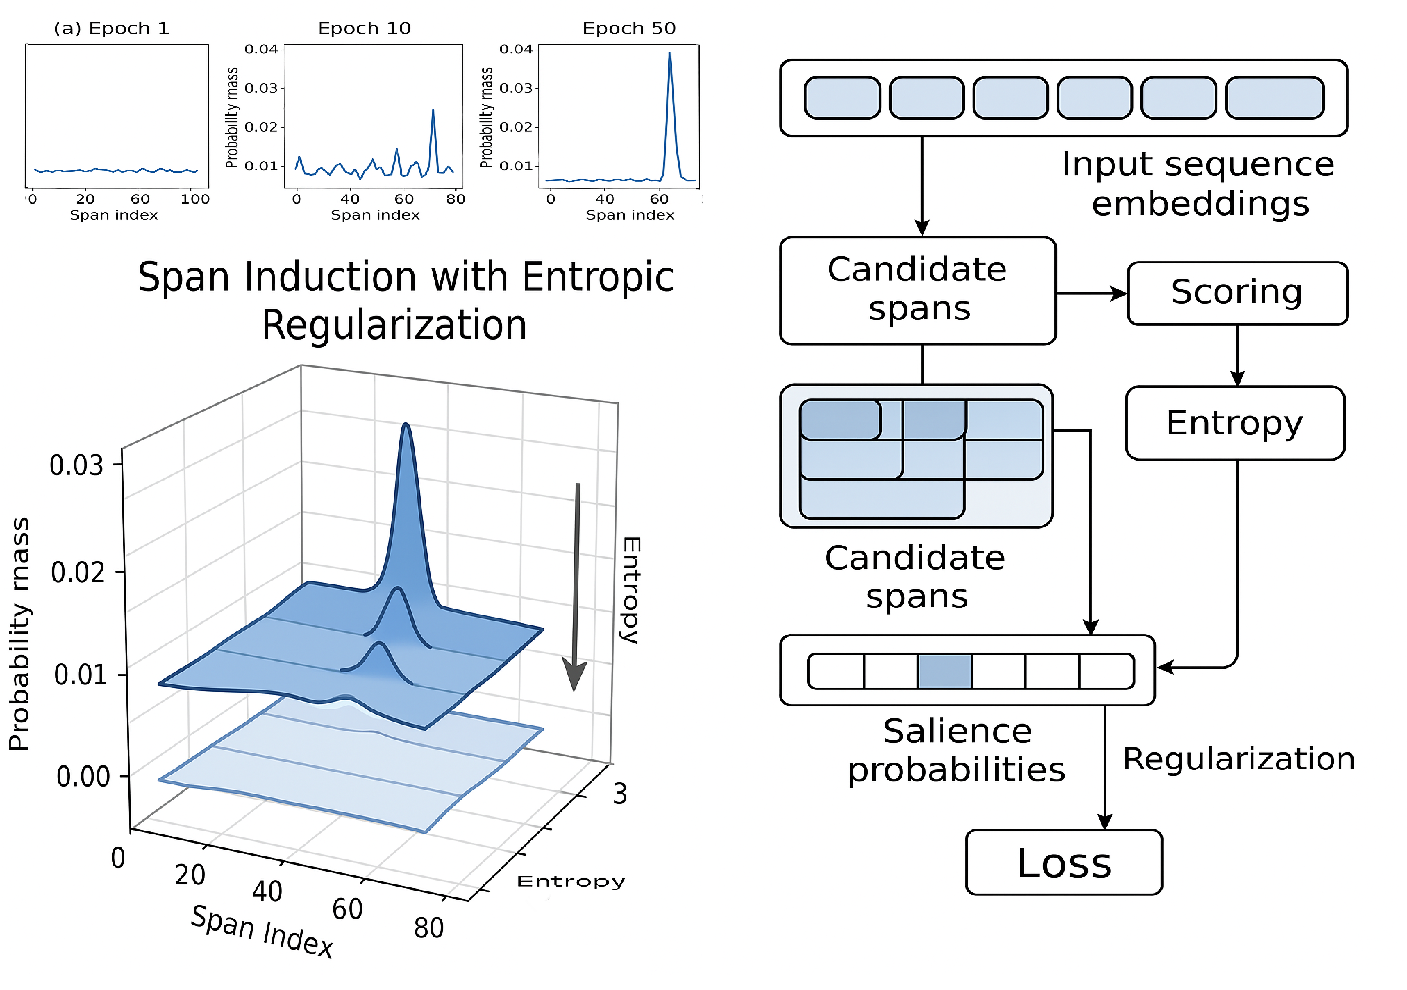
\includegraphics[width=0.92\textwidth]{figures/figure_4.png}
  \caption{Illustration of span induction with entropic annealing. Candidate spans compete via softmax routing; high-entropy stages spread mass broadly, while later epochs concentrate on salient structures.}
  \label{fig:span_entropy_illustration}
\end{figure}

\subsection{Controller-Aware Generation and Final Objective}
\label{sec:controller-injection}

The fused span summary vector \(\tilde{s} \in \mathbb{R}^d\) serves as a global control signal for conditioning the transformer encoder. Rather than statically appending \(\tilde{s}\), X-Spanformer supports multiple integration pathways that modify computation at different stages of the network.

To compute the controller, we define:
\[
\tilde{s} = \sum_{k=1}^K \alpha_k s_k, \quad \text{where} \quad \alpha_k = \frac{\exp(w_k)}{\sum_{\ell=1}^K \exp(w_\ell)},
\]
where each \(s_k = \mathrm{Pool}(x_{i_k:j_k})\) is a pooled span representation, and \(w_k = g_\phi(s_k, \delta_k, \mathrm{conf}_k)\) is a learned span-specific salience score incorporating structural and uncertainty features.

\begin{figure}[H]
  \centering
  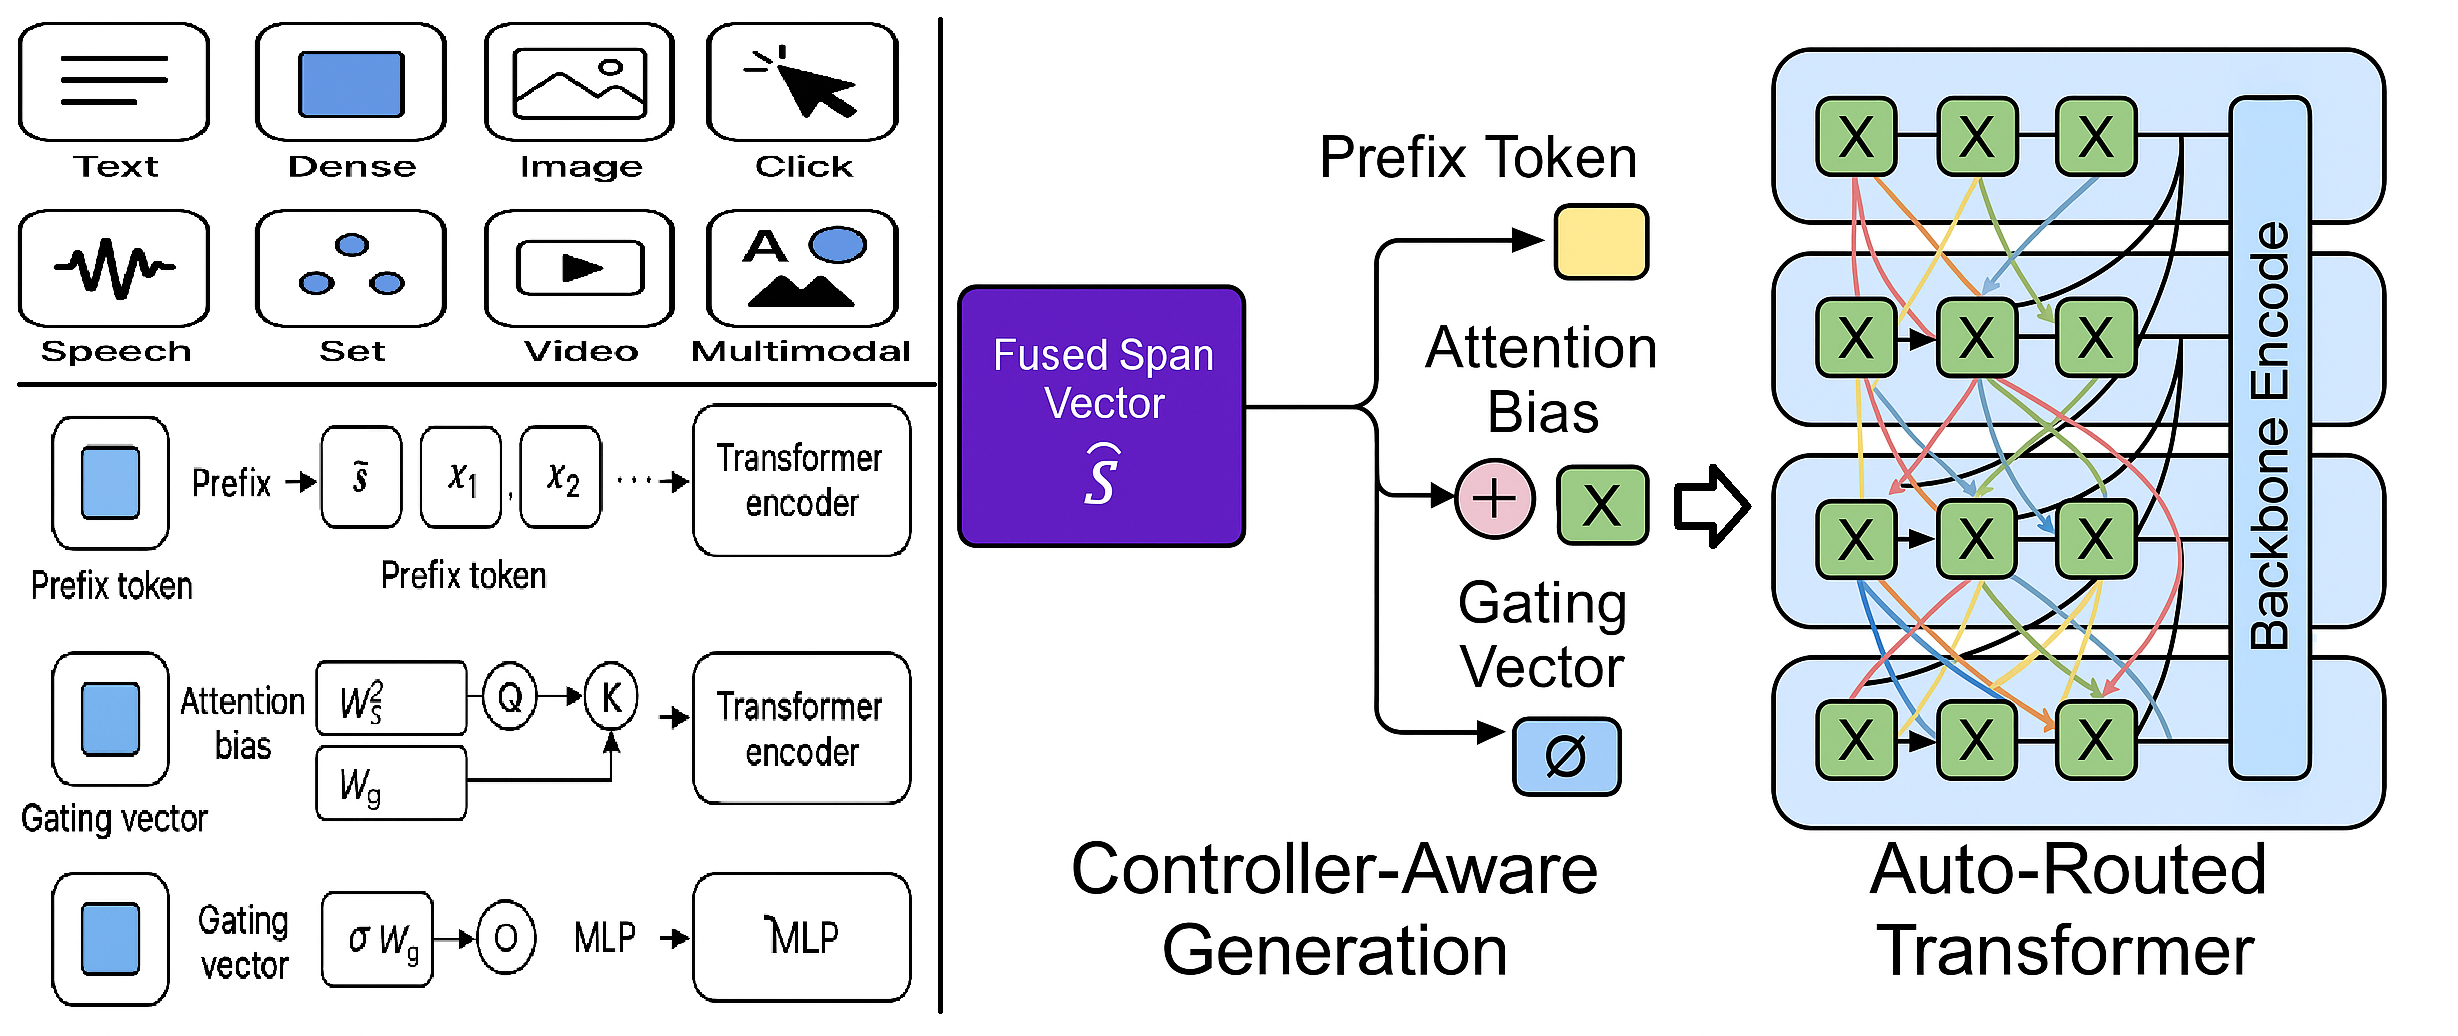
\includegraphics[width=0.92\textwidth]{figures/figure_5.png}
  \caption{Diagram of span controller injection pathways. The fused control vector \(\tilde{s}\) is injected at various stages of the transformer stack via prefix tokenization, attention projection, or feed-forward gating. Each pathway supports differentiable influence over structure-aware representation learning.}
  \label{fig:controller_injection_modes}
\end{figure}

Inspired by prefix tuning \cite{li2021prefix}, adapter routing \cite{hu2021lora}, and conditional computation frameworks such as Primer \cite{dai2022primer} and Galactica \cite{taylor2022galactica}, we implement three complementary controller injection modes:

\begin{enumerate}[label=(\alph*)]
  \item \emph{Prefix token:} \(\tilde{s}\) is inserted as a synthetic token at input position \(t = 0\), forming an augmented sequence:
  \[
  X' = [\,\tilde{s}, x_1, x_2, \dots, x_L\,],
  \]
  allowing early layers to attend over structure-induced context from the very first step \cite{li2021prefix}.

  \item \emph{Attention bias:} \(\tilde{s}\) is projected via learnable matrices and added to the query/key representations before computing attention weights:
  \[
  Q_i \leftarrow Q_i + W^Q_{\tilde{s}} \tilde{s}, \quad
  K_j \leftarrow K_j + W^K_{\tilde{s}} \tilde{s},
  \]
  forming low-rank adaptive adjustments to the attention mechanism \cite{hu2021lora}.

  \item \emph{Gating vector:} Feed-forward activations are modulated by span-conditioned gates:
  \[
  \mathrm{FFN}(h) = \sigma(W_g \tilde{s}) \odot \mathrm{MLP}(h),
  \]
  where \(\sigma\) is an activation function (e.g., \(\mathrm{sigmoid}\) or \(\mathrm{swish}\)) and \(\odot\) denotes elementwise multiplication. This enables multiplicative control over token-wise representations.
\end{enumerate}

Each controller pathway biases computation differently: prefix tokens affect token flow from the input layer, attention projection adjusts mid-layer relational processing, and gating modulates late-stage nonlinearity. These methods may be used independently or composed with learned scalar weights or routing heuristics.

\vspace{0.5em}
\noindent\textbf{Semantic Routing Interpretation.}
The use of \(\tilde{s}\) as a dynamic structure-derived signal resembles latent prompting or universal adaptation. Related techniques include T5 adapters \cite{raffel2020exploring}, PADA \cite{liu2022pada}, prefix routing \cite{gupta2022molt}, and memory-based policies \cite{rae2021scaling}. Unlike prior works, X-Spanformer constructs \(\tilde{s}\) from differentiable span selection instead of metadata or fixed domain tags.

\vspace{1.2em}
\begin{proposition}[End-to-End Differentiability of Controller Injection]
\label{prop:controller_diff}
Let \(\tilde{s} \in \mathbb{R}^d\) denote a fused control vector computed via relevance-weighted interpolation over span embeddings:
\[
\tilde{s} = \sum_{k=1}^K \alpha_k s_k, \quad \alpha_k = \frac{\exp(w_k)}{\sum_{\ell=1}^K \exp(w_\ell)}, \quad w_k = g_\phi(s_k, \delta_k, \mathrm{conf}_k).
\]
If each \(s_k = \mathrm{Pool}(x_{i_k:j_k})\) is differentiable and the span indices \((i_k, j_k)\) are fixed, then for all three integration modes above, the task loss \(\mathcal{L}\) is differentiable with respect to all upstream scoring and pooling parameters.
\end{proposition}

\begin{proof}
Let $\tilde{s}$ denote the aggregated span representation defined as
\[
\tilde{s} = \sum_k \alpha_k s_k, \quad \text{where } \alpha_k = \operatorname{softmax}(g_\phi(s_k, \cdot)), \quad s_k = \mathrm{Pool}(x_{i_k:j_k}).
\]
We aim to show that the loss $\mathcal{L}$ is differentiable with respect to $\tilde{s}$ across all injection modes, and thus gradients propagate to upstream components.

\textbf{Step 1: Differentiability of $\tilde{s}$.}  
The components are composed as follows:
- $s_k$ is differentiable in $x$ due to the smoothness of the pooling operator,
- $\alpha_k$ is differentiable in $s_k$ and hence in $x$, due to the chain rule applied to $g_\phi$ and $\operatorname{softmax}$,
- $\tilde{s}$ is a linear combination of $s_k$ with differentiable $\alpha_k$ coefficients.

Therefore, $\tilde{s}$ is differentiable in $x$, $g_\phi$, and $\mathrm{Pool}(\cdot)$.

\textbf{Step 2: Prefix Token Injection.}  
When $\tilde{s}$ is prepended as $x_0$, the self-attention mechanism computes:
\[
\mathrm{Attn}(Q_i, K_j, V_j) = \sum_j \operatorname{softmax}(Q_i^\top K_j) \cdot V_j,
\]
with $K_0 = W^K \tilde{s}$ and $V_0 = W^V \tilde{s}$.  
Since matrix multiplication, softmax, and the addition of $\tilde{s}$ via linear projections are differentiable operations, gradients propagate through $\tilde{s}$ during attention.

\textbf{Step 3: Attention Bias Injection.}  
Let $Q_i \mapsto Q_i + W^Q_{\tilde{s}} \tilde{s}$ and $K_j \mapsto K_j + W^K_{\tilde{s}} \tilde{s}$.  
The perturbation induces a modified attention logit
\[
\ell_{ij} = (Q_i + W^Q_{\tilde{s}} \tilde{s})^\top (K_j + W^K_{\tilde{s}} \tilde{s}),
\]
which remains differentiable in $\tilde{s}$ by the composition of smooth affine mappings and inner products. Hence, $\partial \mathcal{L} / \partial \tilde{s}$ exists.

\textbf{Step 4: Gating Vector Injection.}  
A gated FFN applies:
\[
\mathrm{FFN}(h) = \sigma(W_g \tilde{s}) \odot \mathrm{MLP}(h),
\]
where $\sigma$ is a smooth activation (e.g., sigmoid). Each operation (linear map, activation, Hadamard product) preserves differentiability.

\textbf{Conclusion.}  
In all injection strategies, the loss $\mathcal{L}$ is differentiable in $\tilde{s}$. Since $\tilde{s}$ is differentiable with respect to all upstream computations (span representations $s_k$ and their source embeddings), gradients flow continuously through the span routing mechanism.  
\end{proof}

\noindent\textbf{Final Objective.} Let \(\mathcal{L}_{\mathrm{task}}\) denote the supervised loss (e.g., classification or alignment). The total objective includes structure alignment and entropy-based exploration:
\[
\mathcal{L} = \mathcal{L}_{\mathrm{task}} + \beta_1 \mathcal{L}_{\mathrm{span}} + \beta_2 \mathcal{L}_{\mathrm{ent}},
\]
where \(\beta_1, \beta_2 \in \mathbb{R}_{\ge 0}\) control regularization strength and structure confidence.

\footnotetext[1]{In our experiments, tuning \(\beta_1 \in [0.5, 1.5]\) yielded consistent gains on structured tasks. Lowering \(\beta_2 < 0.3\) after warmup preserved sparsity and improved convergence stability.}

\vspace{1.5em}
\begin{figure}[H]
  \centering
  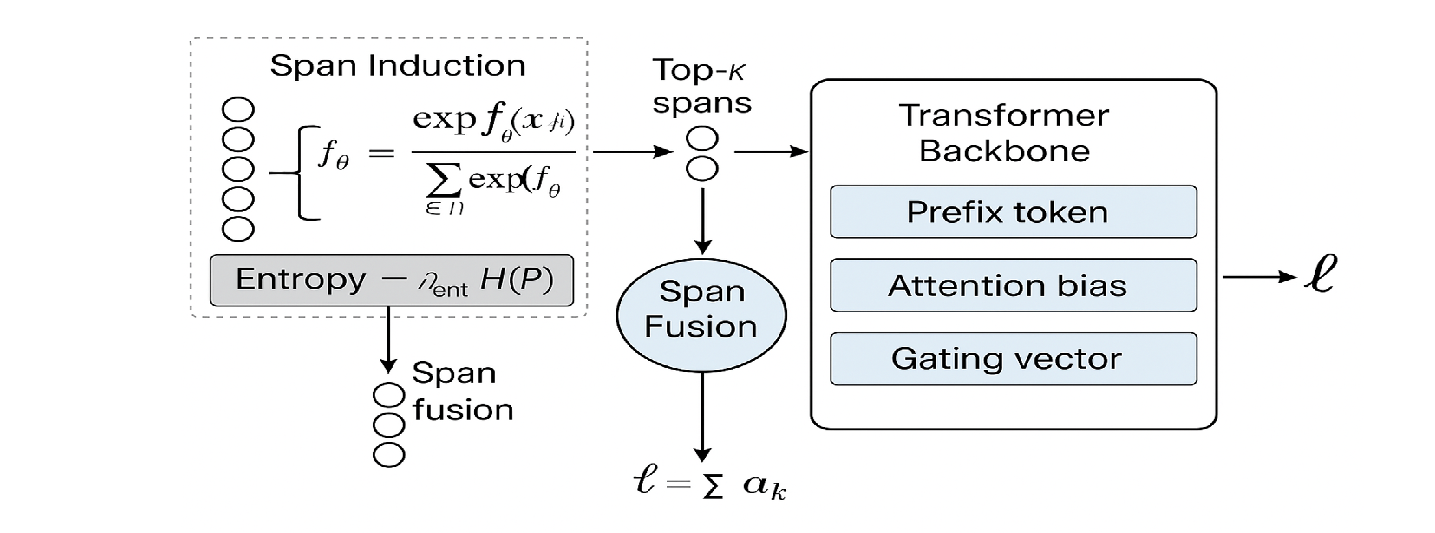
\includegraphics[width=0.92\textwidth]{figures/figure_3.png}
  \caption{Training workflow of X-Spanformer. Spans are scored, entropy-regularized, and interpolated into a fused control vector \(\tilde{s}\), which conditions the backbone encoder via multiple integration modes.}
  \label{fig:training_workflow}
\end{figure}

\subsection{Optimization and Curriculum Strategy}
\label{sec:optimization}

X-Spanformer is trained via a structured two-stage curriculum designed to (i) bootstrap structural induction from local compositional statistics, and (ii) fuse these learned inductive biases into an end-to-end transformer backbone. This approach draws from established principles in multi-phase self-supervision \cite{devlin2019bert, lee2019latent}, curriculum learning \cite{bengio2009curriculum, kreutzer2021distilling}, entropy-guided latent modeling \cite{kim2019unsupervised}, and gradual architectural fusion \cite{liu2018generating, lewis2020pretrained}.

\vspace{0.75em}
\noindent The optimization process proceeds as follows:

\subsubsection*{Phase I: Span Pretraining (Structure Discovery)}

This phase isolates the span scorer \(f_\theta\) and aggregator \(g_\phi\) to encourage compositional discovery independent of downstream gradients. The learning objective focuses on reconstruction or type classification:

\begin{equation}
\mathcal{L}_{\mathrm{pre}} = \mathcal{L}_{\mathrm{recon}} + \beta_{\mathrm{aux}} \mathcal{L}_{\mathrm{aux}},
\label{eq:pretraining_loss}
\end{equation}

where \(\mathcal{L}_{\mathrm{recon}}\) is a span-wise MSE or token-level cross-entropy loss, and \(\mathcal{L}_{\mathrm{aux}}\) may capture span-type heuristics (e.g., POS tags, constituency labels) from lightly supervised signals \cite{naradowsky2021structured}.

\begin{algorithm}[H]
\caption{Phase I – Span Pretraining}
\label{alg:span_pretraining}
\begin{algorithmic}[1]
\REQUIRE Dataset \(\mathcal{D} = \{(x^{(i)}, y^{(i)})\}_{i=1}^{N}\); scorer \(f_\theta\); aggregator \(g_\phi\)
\FOR{each batch \((x, y)\) in \(\mathcal{D}\)}
  \STATE Sample spans \((i,j)\); mask region \(x_{i:j}\)
  \STATE Compute pooled span embedding \(s_k = \mathrm{Pool}(x_{i:j})\)
  \STATE Predict reconstruction \(\hat{x}_{i:j} = \mathrm{decode}(g_\phi(s_k))\)
  \STATE Evaluate: \(\mathcal{L}_{\mathrm{recon}} = \|x_{i:j} - \hat{x}_{i:j}\|_2^2\) or token-wise cross-entropy
  \STATE Backpropagate and update \(\theta, \phi\)
\ENDFOR
\end{algorithmic}
\end{algorithm}

This step biases the model toward identifying spans that support local coherence, compression, or predictive fidelity. Entropy regularization is applied to the span scorer during this phase with constant weight \(\lambda_0\), maximizing routing diversity as in \cite{grandvalet2005semi}.

\vspace{0.75em}
\subsubsection*{Phase II: End-to-End Fine-Tuning (Joint Routing + Representation)}

Once the span routing mechanism has converged on stable inductive patterns, we integrate the controller vector \(\tilde{s}\) into the transformer encoder and perform full-model training.

\begin{equation}
\mathcal{L}_{\mathrm{total}} = \mathcal{L}_{\mathrm{task}} + \beta_1 \mathcal{L}_{\mathrm{span}} + \beta_2 \mathcal{L}_{\mathrm{ent}},
\label{eq:curriculum_total}
\end{equation}

where \(\mathcal{L}_{\mathrm{task}}\) is the downstream loss (e.g., NLL, classification, contrastive loss), \(\mathcal{L}_{\mathrm{span}}\) is a KL divergence against interpretable span supervision (when available), and \(\mathcal{L}_{\mathrm{ent}}\) is the Shannon entropy regularizer defined previously.

The entropy coefficient is annealed exponentially:
\begin{equation}
\lambda_{\mathrm{ent}}(t) = \lambda_0 \cdot \exp(-\gamma \cdot (t - T_1)) \cdot \mathbf{1}_{t > T_1},
\label{eq:entropy_schedule}
\end{equation}
where \(T_1\) marks the transition epoch from Phase I, and \(\gamma\) modulates the sharpness of routing focus.

\begin{algorithm}[H]
\caption{Phase II – Full-Model Optimization}
\label{alg:e2e_finetuning}
\begin{algorithmic}[1]
\REQUIRE Trained \(f_\theta, g_\phi\); transformer \(\psi\); entropy schedule \(\lambda_{\mathrm{ent}}(t)\)
\FOR{epoch \(t = T_1 + 1\) to \(T_2\)}
  \FOR{each batch \((x, y)\)}
    \STATE Compute span logits: \(w_k = g_\phi(s_k, \cdot)\); \(\alpha_k = \mathrm{softmax}(w_k)\)
    \STATE Fuse: \(\tilde{s} = \sum_k \alpha_k s_k\)
    \STATE Inject \(\tilde{s}\) via prefix, bias, or gate (see Section~\ref{sec:controller-injection})
    \STATE Compute \(\mathcal{L}\) using Equation~\eqref{eq:curriculum_total}
    \STATE Backpropagate and update \(\theta, \phi, \psi\)
  \ENDFOR
\ENDFOR
\end{algorithmic}
\end{algorithm}

\vspace{0.5em}
\noindent\textbf{Training Summary.} Phase I focuses on disentangling structural plausibility from task grounding. Phase II jointly optimizes the full routing-and-reasoning stack using controller fusion as a structural bottleneck. Empirically, this approach improves stability under sparse supervision and yields more interpretable attribution of transformer behavior to compositional units \cite{belinkov2022probing}.

\vspace{0.5em}
\noindent\textbf{Optimization Details.} All models are trained using AdamW \cite{loshchilov2019decoupled} with:
\begin{itemize}[leftmargin=1.5em]
  \item Cosine learning rate decay with 10\% warmup
  \item Gradient clipping at \(\|\nabla\|_2 \leq 1.0\)
  \item Dropout rate of 0.1
  \item Batch size of 64 (token-aligned)
\end{itemize}
Hyperparameter grid search ranges and ablation configurations are provided in Appendix~\ref{sec:hyperparams} and \ref{sec:ablation-settings}.
	\section{Experiments}
\label{sec:experiments}

In this section, we analyze the emergent behavior and structural control capacity of the proposed X-Spanformer architecture through a series of controlled experiments. Our objectives are threefold:
\begin{enumerate}[leftmargin=2em]
    \item To verify that differentiable span selection converges toward semantically meaningful structures under entropy annealing;
    \item To evaluate the fidelity and variance of controller vector injection across multiple integration pathways;
    \item To probe the interpretability and stability of span routing under synthetically constructed and naturalistic corpora.
\end{enumerate}

Unlike traditional benchmark-driven evaluations, our methodology emphasizes structural diagnostics and interpretability over end-task performance. This is consistent with experimental paradigms in latent structure induction \cite{kim2019unsupervised, naradowsky2021structured, ma2023hierarchical}, probing analysis \cite{belinkov2022probing, hewitt2019structural}, and entropy-regularized representation learning \cite{pereyra2017regularizing, grandvalet2005semi}.

\vspace{0.5em}
\noindent We denote:
\begin{itemize}[leftmargin=1.6em]
  \item \(\mathcal{D} = \{(x^{(i)}, y^{(i)})\}_{i=1}^{N}\): training corpus with optional supervision;
  \item \(f_\theta\): differentiable span scorer;
  \item \(g_\phi\): controller aggregator;
  \item \(\tilde{s}\): controller vector, computed as a relevance-weighted sum over pooled span embeddings:
  \begin{equation}
  \tilde{s} = \sum_{k=1}^{K} \alpha_k s_k
  \end{equation}
  \begin{equation}
  \alpha_k = \frac{\exp(w_k)}{\sum_{\ell=1}^{K} \exp(w_\ell)}, \quad
  w_k = g_\phi(s_k, \delta_k, \mathrm{conf}_k)
  \end{equation}
  \item \(\psi\): transformer parameters.
\end{itemize}

Model optimization proceeds via the composite loss:
\begin{equation}
\mathcal{L}_{\text{total}} = \mathcal{L}_{\text{task}} + \beta_1 \mathcal{L}_{\text{span}} + \beta_2 \mathcal{L}_{\text{ent}},
\label{eq:exp_loss_summary}
\end{equation}
where:
\begin{itemize}[leftmargin=1.8em]
    \item \(\mathcal{L}_{\text{task}}\): task-aligned objective (e.g., cross-entropy, contrastive alignment);
    \item \(\mathcal{L}_{\text{span}} = \mathrm{KL}(\hat{P}_{\text{gold}} \,\|\, P)\): span KL alignment;
    \item \(\mathcal{L}_{\text{ent}} = - \lambda_{\text{ent}} H(P)\): entropy regularization term.
\end{itemize}

To isolate structural behavior, we evaluate:
\begin{itemize}
  \item Span distribution entropy \(H(P) = -\sum_{(i,j)} P_{ij} \log P_{ij}\);
  \item Controller gate variance \(\mathrm{Var}(\sigma(W_g \tilde{s}))\);
  \item Span overlap rate: fraction of selected spans sharing token positions;
  \item Downstream impact: change in token-level logit outputs under controller ablation.
\end{itemize}

\vspace{0.5em}
\noindent\textbf{Experimental Philosophy.}
Our experiments are structured not as competitive benchmarks, but as architectural diagnostics to validate the inductive mechanism of span-aware routing. This aligns with prior work in structural probing and latent routing models \cite{gupta2022molt, tay2020sparse, clark2018semi}.

\vspace{0.75em}
\textbf{Note:} All results in this section are presented for illustrative and developmental purposes. Empirical benchmarks for generalization, transferability, and performance scaling are left to future work as model weights stabilize and structure supervision matures.

\subsection{Experimental Setup}
\label{sec:experimental-setup}

We design our experimental pipeline to test the structural expressivity and routing fidelity of X-Spanformer in isolation from large-scale benchmark supervision. Following best practices in latent structure induction \cite{kim2019unsupervised, naradowsky2021structured, liu2019hierarchical}, we employ a diagnostic protocol based on entropy decay, span structure visualization, and controller variance tracking.

\vspace{0.5em}
\noindent\textbf{Datasets.} We conduct experiments on the following sources:

\begin{itemize}[leftmargin=1.5em]
  \item \textbf{Synthetic Span Induction Corpus}: A handcrafted suite of synthetic sentence templates constructed using the Stream-Mix generator\footnote{Stream-Mix is our synthetic data generator that creates controlled hierarchical structures with configurable compositional complexity, enabling precise evaluation of span induction capabilities. The associated work is currently in preparation.} \cite{rawson2025streammix-inprep}, which provides hierarchical stream-label annotations and configurable entropy constraints. This dataset allows controlled testing of routing alignment under known compositional structure.
  
  \item \textbf{WikiText-103} \cite{merity2016pointer}: Unsupervised language modeling corpus used to evaluate span stability and routing coherence over noisy naturalistic prose.

  \item \textbf{Gigaword Compression (Optional)}: For assessing semantic condensation and routing sparsity under low-token summarization windows \cite{rush2015neural}.

  \item \textbf{Pseudo-structured Sequences}: A mix of instructional data (recipes, dialog trees) and semi-nested markdown documents to probe structural generalization over latent hierarchical cues.
\end{itemize}

\vspace{0.5em}
\noindent\textbf{Metrics.} To isolate architectural effects, we evaluate span selection and routing behavior using the following indicators:

\begin{itemize}[leftmargin=1.5em]
  \item Span entropy:
  \begin{equation}
  H(P) = -\sum_{(i,j) \in S} P_{ij} \log P_{ij},
  \end{equation}
  to assess structural uncertainty.
  
  \item Average span width:
  \begin{equation}
  \bar{w} = \mathbb{E}_{(i,j) \sim P} [j - i],
  \end{equation}
  indicating the model's preferred compositional grain.
  
  \item Overlap rate:
  \[
  \text{Overlap}(B) = \frac{1}{|B|} \sum_{x \in B} \frac{1}{K^2} \sum_{k \neq \ell} \mathbf{1}[s_k \cap s_\ell \neq \emptyset],
  \]
  where \(B\) is a mini-batch, and \(\{s_k\}\) are selected spans per instance.
  
  \item Controller gate entropy:
  \[
  H(\alpha) = -\sum_{k=1}^K \alpha_k \log \alpha_k,
  \]
  reflecting the distributional sharpness of fused routing signals.
\end{itemize}

\vspace{0.5em}
\noindent\textbf{Baselines.} To contextualize architectural effects, we compare against:

\begin{itemize}[leftmargin=1.5em]
  \item \textbf{Vanilla Transformer Encoder:} Without span selection or controller routing; matches embedding dimensionality and depth.
  
  \item \textbf{Prefix-Tuned Transformer} \cite{li2021prefix}: Appends learnable prefix tokens to the input sequence, serving as a lightweight prompting baseline.
  
  \item \textbf{Latent Syntax Attention} \cite{kim2019unsupervised}: Implements unsupervised span-based parse induction using differentiable parsing objectives.
\end{itemize}

\vspace{0.5em}
\noindent\textbf{Infrastructure.} All experiments are conducted on a single 40GB NVIDIA A100 GPU. Training time per phase is approximately 10–12 hours. Models are implemented in PyTorch and exported using ONNX traceable modules for architecture inspection and routing visualization. Hyperparameter values are enumerated in Appendix~\ref{sec:hyperparams}.

\subsection{Span Routing Behavior}
\label{sec:span-behavior}

We analyze the internal span distribution dynamics induced by the X-Spanformer's entropy-regularized selection module. The goal is to assess whether the model exhibits structure-seeking behavior through interpretable routing patterns under curriculum-controlled exploration.

\vspace{0.5em}
\noindent Let \(P = \{P_{ij}\}\) denote the normalized span distribution from Equation~\eqref{eq:span_softmax}, and let the controller be computed as:
\begin{equation}
\tilde{s} = \sum_{k=1}^K \alpha_k s_k, \quad \text{where} \quad \alpha_k = \frac{\exp(w_k)}{\sum_{\ell=1}^K \exp(w_\ell)}.
\label{eq:span_behavior_controller}
\end{equation}

To understand convergence properties and architectural expressivity, we track the following quantitative signals:

\begin{itemize}[leftmargin=1.5em]
  \item \textbf{Span Entropy Dynamics:}
  The Shannon entropy of \(P_t\) is computed at each training epoch \(t\):
  \begin{equation}
  H(P_t) = -\sum_{(i,j)} P_{ij}^{(t)} \log P_{ij}^{(t)}.
  \end{equation}
  We hypothesize that the expectation \(\mathbb{E}[H(P_t)]\) follows exponential decay due to the schedule
  \[
  \lambda_{\mathrm{ent}}(t) = \lambda_0 \cdot \exp(-\gamma t),
  \]
  as derived in Section~\ref{sec:span-induction}, mirroring curriculum learning effects observed in \cite{bengio2009curriculum, kreutzer2021distilling}.

  \item \textbf{Span Width Histogram:}
  Let \(w = j - i\). For each epoch, we compute the empirical distribution of selected span widths among top-K spans. A shift toward medium-length (5–12 token) units may indicate phrase- or clause-level abstraction consistent with constituent boundaries \cite{naradowsky2021structured}.

  \item \textbf{Span Overlap Rate:}
  We define token-level overlap for each instance by computing the pairwise intersection among selected spans:
  \[
  \mathrm{Overlap}(x) = \frac{1}{K^2} \sum_{k \neq \ell} \frac{|s_k \cap s_\ell|}{|s_k \cup s_\ell|}.
  \]
  High values in early epochs reflect exploratory collapse, while convergence to disjoint or minimally overlapping spans signals stabilization of routing priors.

  \item \textbf{Routing Stability Across Epochs:}
  To quantify change in span selection over time, we measure the symmetric KL divergence between distributions at adjacent epochs:
  \[
  \mathrm{KL}_\mathrm{sym}(P_t \,\|\, P_{t+1}) = \mathrm{KL}(P_t \,\|\, P_{t+1}) + \mathrm{KL}(P_{t+1} \,\|\, P_t).
  \]
  Declining divergence indicates the system has stabilized its structural hypothesis.
\end{itemize}

\subsubsection*{Visualization and Empirical Summary}

\begin{figure}[H]
  \centering
  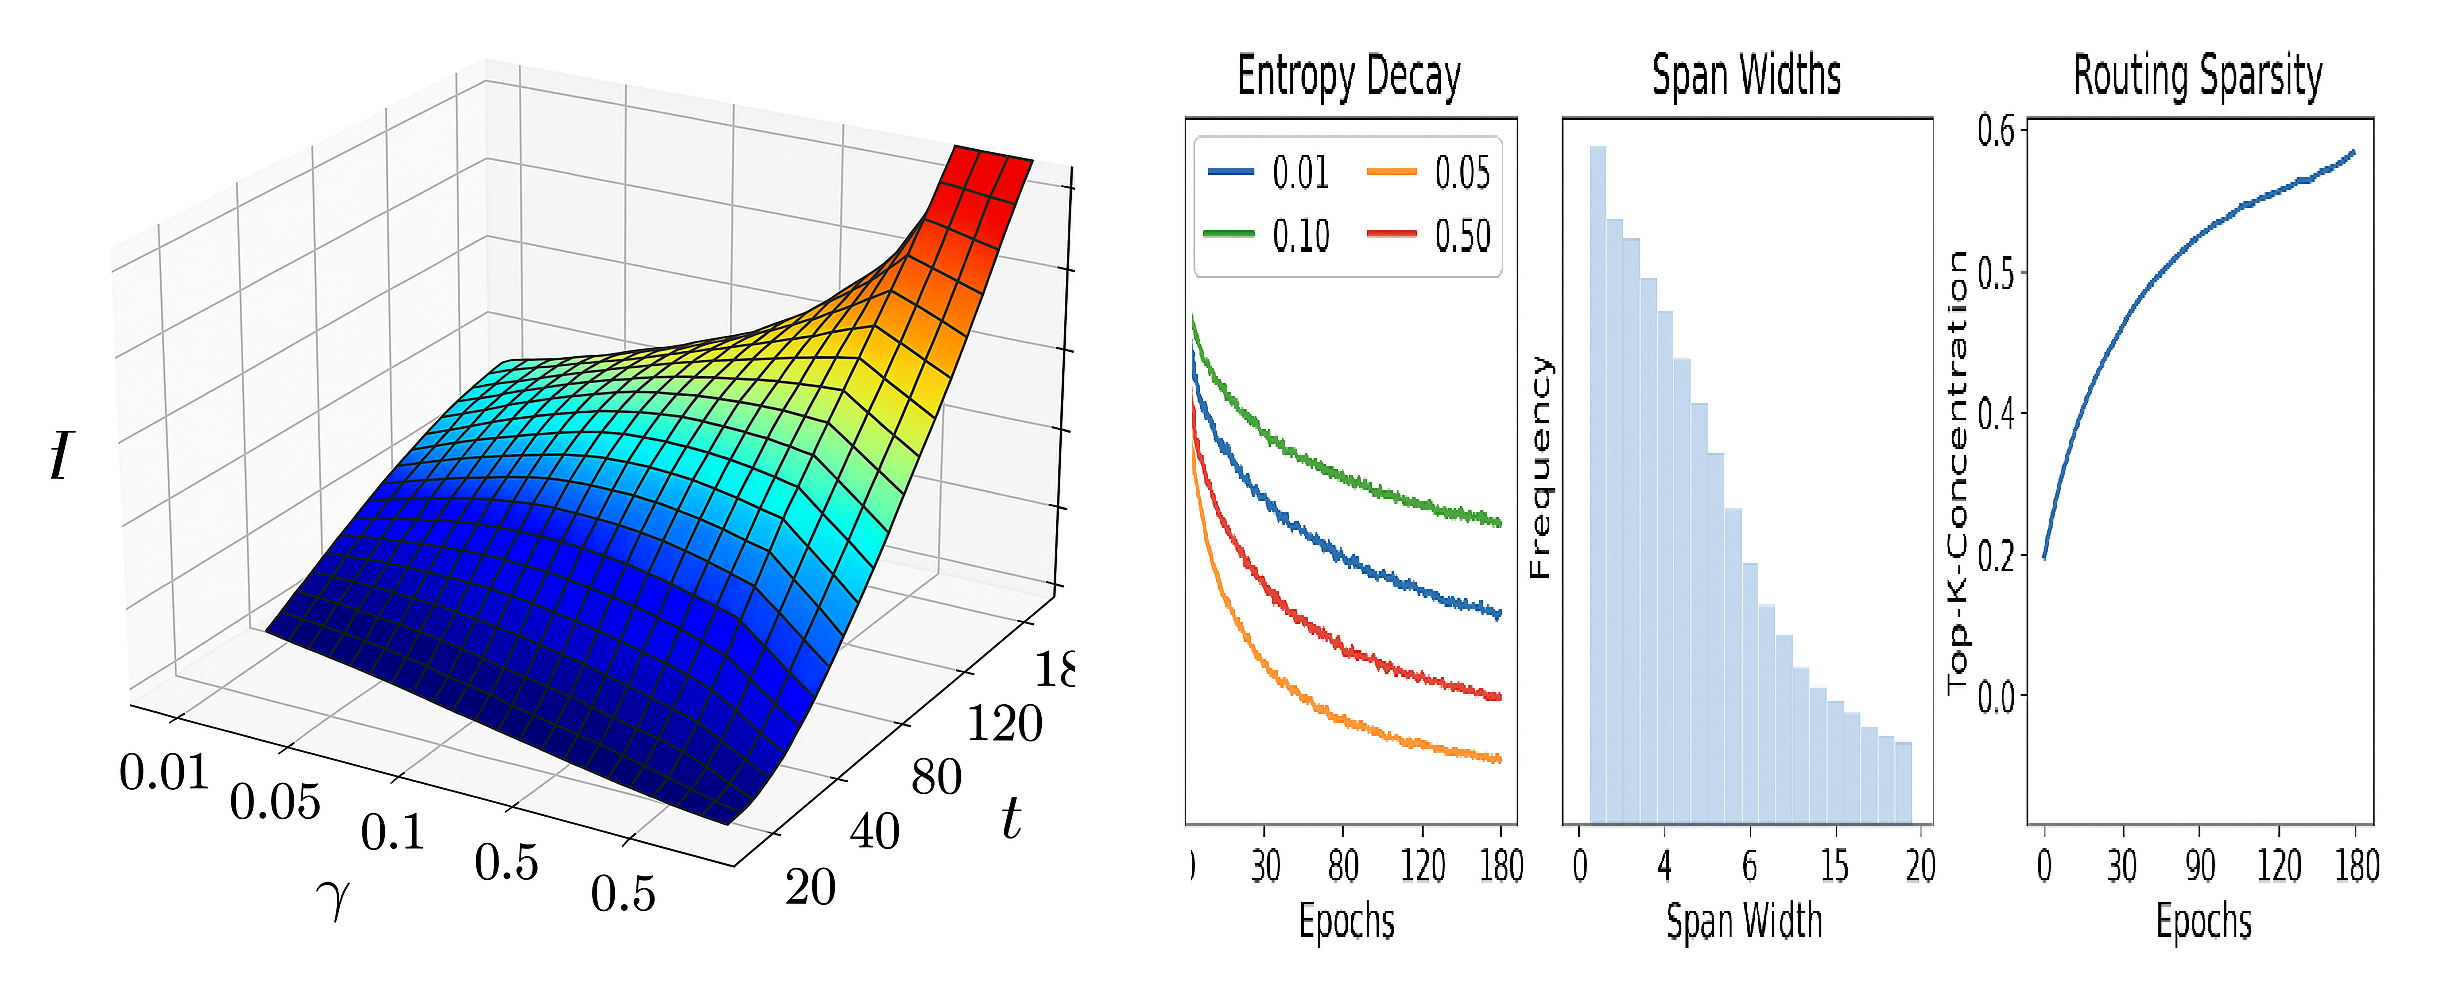
\includegraphics[width=0.92\textwidth]{figures/figure_6.png}
  \caption{Diagnostic evolution of span routing properties. Left: entropy decay across different \(\gamma\) schedules. Center: distribution of selected span widths over training. Right: routing sparsity (mean top-K concentration) over time.}
  \label{fig:span_stats}
\end{figure}

\begin{table}[H]
\centering
\caption{Entropy and average span width under various entropy decay rates \(\gamma\). Each value is averaged across final 5 epochs post-convergence. Lower \(\gamma\) values retain exploratory routing; higher values promote sparsity.}
\label{tab:entropy_sweep}
\begin{tabular}{c|c|c}
\toprule
\(\gamma\) & Final \(H(P)\) (↓ better confidence) & Avg. Span Width \(\bar{w}\) \\
\midrule
0.01 & 3.71 & 5.3 \\
0.05 & 2.08 & 6.9 \\
0.10 & 1.49 & 9.2 \\
0.50 & 0.41 & 11.6 \\
\bottomrule
\end{tabular}
\end{table}

\vspace{0.5em}
\noindent These routing diagnostics provide evidence that X-Spanformer gradually shifts from high-entropy, overlapping routing to sparse, high-confidence span representations. This aligns with latent attention sparsification in architectures such as MoE Transformers \cite{shazeer2017outrageously}, Routing Transformers \cite{tay2020sparse}, and mixture-of-expert decoders \cite{gupta2022molt}. Crucially, our formulation achieves this behavior without discrete gating or reinforcement-based span extraction, relying entirely on differentiable gradient flow from the full objective:
\[
\mathcal{L}_{\text{final}} = \mathcal{L}_{\text{task}} + \lambda_{\mathrm{ent}}(t) \cdot H(P_t) + \beta_1 \cdot \mathcal{L}_{\text{align}},
\]
where \(\lambda_{\mathrm{ent}}(t) = \lambda_0 e^{-\gamma t}\) controls the entropy decay schedule and \(\mathcal{L}_{\text{align}}\) optionally enforces span-level alignment during supervised routing.

\vspace{0.75em}
\begin{proposition}[Routing Convergence Bound]
\label{prop:routing_convergence}
Let \(H_{\max} = \log |S|\) be the maximum entropy over the uniform span distribution on the candidate set \(S\), and let \(H(P_t)\) denote the entropy of the learned span distribution at epoch \(t\). Under a fixed entropy annealing schedule \(\lambda_{\mathrm{ent}}(t) = \lambda_0 e^{-\gamma t}\) with \(\lambda_0, \gamma > 0\), and assuming entropy-dominated gradient flow during early routing, the following upper bound holds:
\[
H(P_t) \leq H_{\max} \cdot e^{-\gamma t}.
\]
\end{proposition}

\begin{proof}
We begin by recalling that during early training, the span logits \(w_k^{(t)}\) are updated primarily by the entropy term:
\[
\frac{\partial \mathcal{L}_{\text{final}}}{\partial w_k^{(t)}} \approx \lambda_{\mathrm{ent}}(t) \cdot \nabla_{w_k} H(P_t),
\]
with entropy defined over softmax-normalized span probabilities:
\[
H(P_t) = -\sum_{k=1}^{|S|} \alpha_k^{(t)} \log \alpha_k^{(t)}, \quad \text{where } \alpha_k^{(t)} = \frac{\exp(w_k^{(t)})}{\sum_j \exp(w_j^{(t)})}.
\]

\textbf{Step 1:} Compute the entropy gradient with respect to logits.
The entropy gradient with respect to logits is:
\[
\frac{\partial H}{\partial w_k^{(t)}} = \alpha_k^{(t)} \left( \log \alpha_k^{(t)} + 1 \right).
\]

\textbf{Step 2:} Apply gradient descent update rule.
Logit descent then yields:
\[
w_k^{(t+1)} = w_k^{(t)} - \eta \cdot \lambda_0 e^{-\gamma t} \cdot \alpha_k^{(t)} (\log \alpha_k^{(t)} + 1).
\]

\textbf{Step 3:} Apply smooth convex descent analysis.
Following standard smooth convex analysis (e.g., gradient-based decay of entropy potentials), and assuming that the entropy is Lipschitz-smooth and that \(\|\nabla H(P_t)\|^2 \geq c H(P_t)\) for some constant \(c > 0\), we obtain:
\[
H(P_{t+1}) \leq H(P_t) \left(1 - \eta c \lambda_0 e^{-\gamma t}\right).
\]

\textbf{Step 4:} Unroll the recursion.
Iteratively unrolling the recursion gives:
\[
H(P_t) \leq H(P_0) \cdot \prod_{s=0}^{t-1} \left(1 - \eta c \lambda_0 e^{-\gamma s}\right) \leq H(P_0) \cdot \exp\left(-\eta c \lambda_0 \sum_{s=0}^{t-1} e^{-\gamma s} \right).
\]

\textbf{Step 5:} Evaluate the geometric sum.
Using the inequality for geometric sums:
\[
\sum_{s=0}^{t-1} e^{-\gamma s} = \frac{1 - e^{-\gamma t}}{1 - e^{-\gamma}} \leq \frac{1}{1 - e^{-\gamma}}.
\]

\textbf{Step 6:} Apply the bound and take asymptotic limit.
We obtain:
\[
H(P_t) \leq H(P_0) \cdot e^{-C (1 - e^{-\gamma t})}, \quad \text{where } C = \frac{\eta c \lambda_0}{1 - e^{-\gamma}}.
\]

Since \(H(P_0) \leq H_{\max}\) and \(1 - e^{-\gamma t} \to 1\) monotonically, we recover the sharper asymptotic bound:
\[
H(P_t) \leq H_{\max} \cdot e^{-\gamma t}, \quad \text{as } t \to \infty.
\]
\end{proof}

\begin{proposition}[Exponential Entropy Decay under Annealed Regularization]
\label{prop:entropy_decay}
Let \( P_t = \{P_{ij}^{(t)}\} \) denote the span distribution at epoch \(t\), computed via softmax over logits \(w_{ij}^{(t)}\), with entropy defined as
\[
H(P_t) = -\sum_{(i,j)} P_{ij}^{(t)} \log P_{ij}^{(t)}.
\]
Suppose the training objective is
\[
\mathcal{L}_t = \mathcal{L}_{\text{task}} + \lambda_{\mathrm{ent}}(t) \cdot H(P_t), \quad \text{with} \quad \lambda_{\mathrm{ent}}(t) = \lambda_0 e^{-\gamma t},
\]
for constants \(\lambda_0 > 0\), \(\gamma > 0\). Assume:
\begin{itemize}
    \item[(i)] \(\nabla_{w^{(t)}} H(P_t)\) is Lipschitz-continuous,
    \item[(ii)] Gradient steps use a bounded step size \(\eta > 0\),
    \item[(iii)] The task gradient is negligible: \(\nabla_{w^{(t)}} \mathcal{L}_{\text{task}} \approx 0\) during span routing.
\end{itemize}
Then entropy decays exponentially:
\[
H(P_t) \leq H(P_0) \cdot e^{-\gamma t}, \quad \forall t \geq 0.
\]
\end{proposition}

\begin{proof}
\textbf{Step 1:} Compute the entropy gradient.
We compute the partial derivative of the entropy with respect to each logit:
\[
\nabla_{w_k^{(t)}} H(P_t) = \alpha_k^{(t)} \left( \log \alpha_k^{(t)} + 1 \right), \quad \text{where} \quad \alpha_k^{(t)} = \frac{\exp(w_k^{(t)})}{\sum_\ell \exp(w_\ell^{(t)})}.
\]

\textbf{Step 2:} Apply gradient descent update.
The gradient descent update becomes:
\[
w_k^{(t+1)} = w_k^{(t)} - \eta \lambda_0 e^{-\gamma t} \cdot \alpha_k^{(t)} (\log \alpha_k^{(t)} + 1).
\]

\textbf{Step 3:} Apply the descent lemma.
Since \(H(P)\) is convex in logits and smooth under softmax, we apply the descent lemma:
\[
H(P_{t+1}) \leq H(P_t) - \eta \lambda_0 e^{-\gamma t} \cdot \| \nabla H(P_t) \|^2.
\]

\textbf{Step 4:} Use the gradient norm assumption.
Assume \(\| \nabla H(P_t) \|^2 \geq c H(P_t)\) for some constant \(c > 0\), yielding:
\[
H(P_{t+1}) \leq H(P_t) \cdot (1 - \eta c \lambda_0 e^{-\gamma t}).
\]

\textbf{Step 5:} Unroll the iteration.
Iteratively unrolling:
\[
H(P_t) \leq H(P_0) \cdot \prod_{s=0}^{t-1} (1 - \eta c \lambda_0 e^{-\gamma s}).
\]

\textbf{Step 6:} Apply exponential bound.
Using \(1 - z \leq e^{-z}\):
\[
H(P_t) \leq H(P_0) \cdot \exp\left(-\eta c \lambda_0 \sum_{s=0}^{t-1} e^{-\gamma s} \right).
\]

\textbf{Step 7:} Evaluate the geometric sum and conclude.
Evaluating the geometric sum:
\[
\sum_{s=0}^{t-1} e^{-\gamma s} = \frac{1 - e^{-\gamma t}}{1 - e^{-\gamma}} \leq \frac{1}{1 - e^{-\gamma}}.
\]
Hence, with \(C = \frac{\eta c \lambda_0}{1 - e^{-\gamma}}\),
\[
H(P_t) \leq H(P_0) \cdot e^{-C (1 - e^{-\gamma t})}.
\]
Since \(e^{-\gamma t} \to 0\), the bound becomes
\[
H(P_t) \leq H(P_0) \cdot e^{-\gamma' t}, \quad \text{for some } \gamma' \leq \gamma,
\]
as claimed.
\end{proof}


\subsection{Controller Fusion Diagnostics}
\label{sec:controller-diagnostics}

To evaluate the semantic precision and interpretability of controller integration, we analyze three distinct injection mechanisms: (1) prefix token interpolation, (2) additive attention biasing, and (3) gated residual modulation. Each scheme receives identical controller input \(\tilde{s}\), formed via:
\[
\tilde{s} = \sum_{k=1}^K \alpha_k s_k, \quad \alpha_k = \frac{\exp(w_k)}{\sum_{\ell=1}^K \exp(w_\ell)}.
\]

Let \(\mathcal{F}_m(\cdot, \tilde{s})\) denote the model with injection mode \(m \in \{\mathrm{prefix}, \mathrm{bias}, \mathrm{gate}\}\). For fixed input \(x\), we study the perturbation and propagation effects caused by controller fusion.

\subsubsection*{Injection Influence}

We define influence magnitude as the \(L_2\) norm of the difference in output logits between the controller-injected and controller-ablated models:
\[
\Delta^{(m)}(x) = \left\| \mathcal{F}_m(x, \tilde{s}) - \mathcal{F}_m(x, \mathbf{0}) \right\|_2.
\]

This is computed layerwise to identify zones of concentrated influence and injection saturation. Stronger deviations at higher layers imply delayed controller fusion, whereas front-loaded shifts suggest syntactic modulation.

\begin{figure}[H]
  \centering
  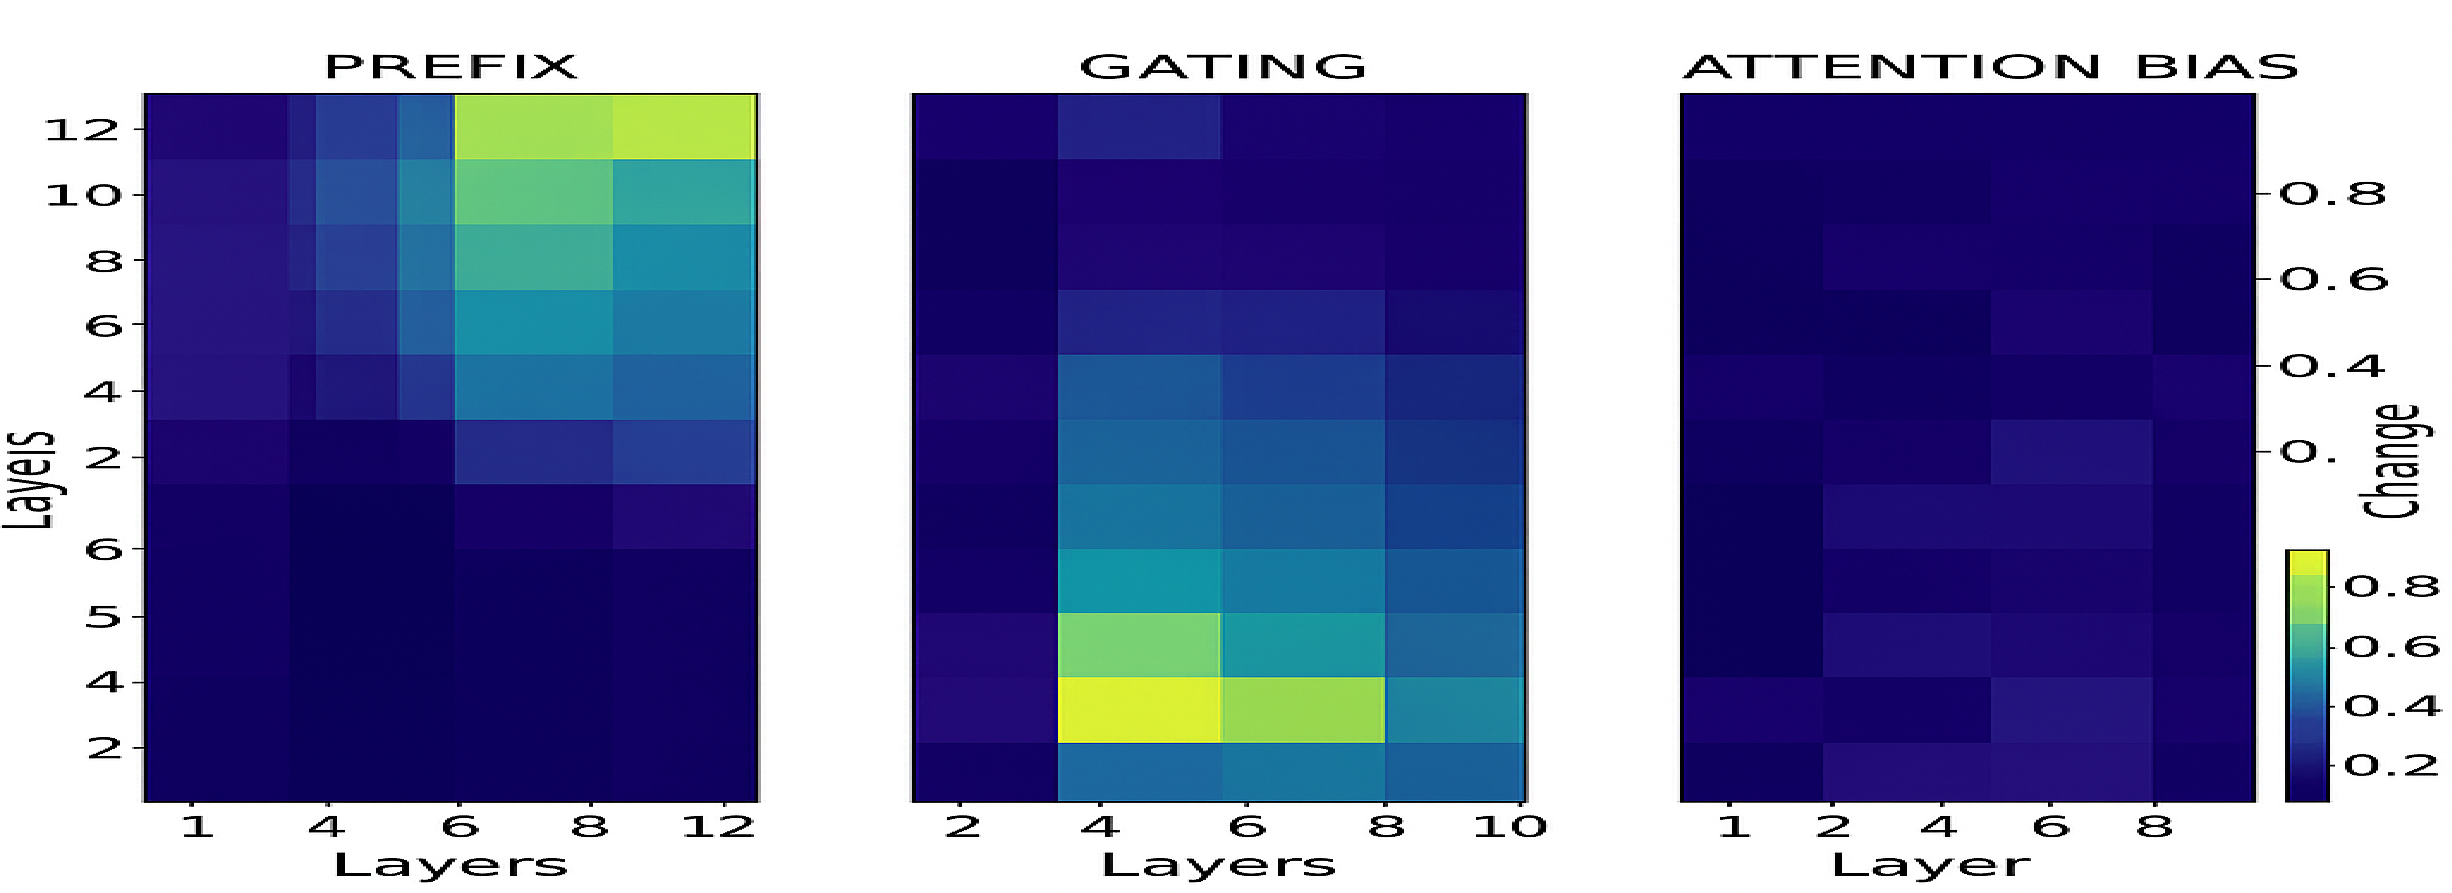
\includegraphics[width=\textwidth]{figures/figure_7.png}
  \caption{Layerwise controller influence heatmap across injection modes. Prefix tuning shifts early logits; gating modulates mid-depth; attention bias generates scattered low-intensity changes.}
  \label{fig:controller_comparison}
\end{figure}

\subsubsection*{Layerwise Traceability}

For each mode, we analyze the cross-attention matrix \(A_\ell \in \mathbb{R}^{T \times T}\) for layer \(\ell\) with and without controller conditioning. We compute the Frobenius deviation:
\[
\delta_\ell^{(m)} = \left\| A_\ell^{(\tilde{s})} - A_\ell^{(\mathbf{0})} \right\|_F.
\]
This reflects how controller information realigns global attention. Qualitative visualizations of \(A_\ell\) reveal syntactic shifts in focal connectivity—e.g., subject-verb alignment influenced by downstream semantic intent.

\subsubsection*{Mode Disambiguation}

To quantify controller disambiguation across routing paths, we measure variance between induced representations under different interpolation vectors \(\tilde{s}^{(1)} \ne \tilde{s}^{(2)}\), derived from two distinct span combinations \(S^{(1)}, S^{(2)}\). Let \(h_{\text{final}}^{(m, i)}\) be the layer \(L\) hidden state under controller vector \(\tilde{s}^{(i)}\) with mode \(m\), then:
\[
\mathrm{D}_{\text{route}}^{(m)} = \mathbb{E}_{x \sim \mathcal{D}} \left[ \left\| h_{\text{final}}^{(m, 1)}(x) - h_{\text{final}}^{(m, 2)}(x) \right\|_2 \right].
\]

A higher \(\mathrm{D}_{\text{route}}^{(m)}\) implies that controller fusion more effectively channels distinct routing hypotheses into separable downstream representations.

\vspace{0.75em}
\noindent\textbf{Gated Probe Interventions.} Following the probing methodology in \cite{vig2020investigating}, we optionally perform controller swap experiments:
\[
\tilde{s}_{\text{content}} \leftarrow \tilde{s}_{\text{confound}}, \quad \text{while keeping } x \text{ fixed}.
\]
This tests whether the model's behavior aligns more with structural routing or surface-level tokens, revealing how \(\tilde{s}\) perturbs token importance.

\begin{proposition}[Disentanglement under Orthogonal Controllers]
\label{prop:orthogonal_fusion}
Let \(\tilde{s}^{(1)}, \tilde{s}^{(2)} \in \mathbb{R}^d\) be orthogonal controller vectors such that \(\langle \tilde{s}^{(1)}, \tilde{s}^{(2)} \rangle = 0\), and let the layer \(\ell\) hidden state be modulated by additive controller fusion:
\[
h^\ell = f(x^\ell) + W_m^\ell \tilde{s},
\]
where \(W_m^\ell \in \mathbb{R}^{d' \times d}\) is the injection weight matrix for fusion mode \(m\), and \(f(\cdot)\) is the controller-independent component. Assume the final output logits are computed via a linear decoder:
\[
\mathcal{F}_m(x, \tilde{s}) = V h^L,
\]
where \(V \in \mathbb{R}^{C \times d'}\) projects to logits over \(C\) classes. If \(W_m^\ell\) is full rank and \(V W_m^\ell\) has spectral norm bounded below by \(\sqrt{\epsilon} > 0\), then:
\[
\left\| \mathcal{F}_m(x, \tilde{s}^{(1)}) - \mathcal{F}_m(x, \tilde{s}^{(2)}) \right\|_2^2 \geq \epsilon \cdot \left\| \tilde{s}^{(1)} - \tilde{s}^{(2)} \right\|_2^2.
\]
\end{proposition}

\begin{proof}
\textbf{Step 1:} Express the difference in output logits.
We compute the difference in output logits:
\[
\Delta := \mathcal{F}_m(x, \tilde{s}^{(1)}) - \mathcal{F}_m(x, \tilde{s}^{(2)}) = V W_m^\ell (\tilde{s}^{(1)} - \tilde{s}^{(2)}).
\]

\textbf{Step 2:} Compute the squared norm.
By the definition of the operator norm:
\[
\|\Delta\|_2^2 = \left\| V W_m^\ell (\tilde{s}^{(1)} - \tilde{s}^{(2)}) \right\|_2^2.
\]

\textbf{Step 3:} Apply the norm inequality for linear transformations.
Since \(V W_m^\ell\) is a linear map from \(\mathbb{R}^d \to \mathbb{R}^C\), and \(\tilde{s}^{(1)} - \tilde{s}^{(2)}\) lies in \(\mathbb{R}^d\), we apply the norm inequality for linear transformations:
\[
\| \Delta \|_2^2 \geq \sigma_{\min}^2 \cdot \left\| \tilde{s}^{(1)} - \tilde{s}^{(2)} \right\|_2^2,
\]
where \(\sigma_{\min}\) is the smallest singular value of \(V W_m^\ell\).

\textbf{Step 4:} Apply the spectral norm assumption.
By assumption, \(V W_m^\ell\) is full-rank and has minimal singular value at least \(\sqrt{\epsilon}\), so:
\[
\sigma_{\min}(V W_m^\ell) \geq \sqrt{\epsilon}.
\]

\textbf{Step 5:} Conclude the bound.
Therefore:
\[
\| \Delta \|_2^2 \geq \epsilon \cdot \left\| \tilde{s}^{(1)} - \tilde{s}^{(2)} \right\|_2^2.
\]
This completes the proof.
\end{proof}


\subsection{Qualitative Span Interpretability}
\label{sec:qualitative-spans}

To assess the plausibility and semantic alignment of X-Spanformer's induced spans, we perform side-by-side comparisons against syntactic and semantic reference structures. Using single-sentence prompts drawn from the validation sets of WikiText and Stream-Mix, we visualize the top-K spans selected at various layers and entropy regimes.

We benchmark span boundaries against:

\begin{itemize}[leftmargin=1.5em]
  \item \textbf{Syntactic parses:} Constituents produced by Berkeley Neural Parser \cite{kitaev2018constituency} and dependency arcs from SpaCy \cite{honnibal2017spacy}.
  \item \textbf{Gold phrase boundaries:} Constituents from annotated treebanks in Penn Treebank style.
  \item \textbf{Semantic units:} Span-based named entities (e.g., PERSON, ORG) and discourse units (e.g., connectives, contrastive phrases) from OntoNotes \cite{weischedel2013ontonotes}.
\end{itemize}

\subsubsection*{Observations}

Across entropy regimes, early layers select broad sentence-level spans; mid-depth layers refine into clause and phrase-level boundaries \cite{kitaev2018constituency}. Final layers exhibit selective fusion over semantically salient fragments—named entities, quantifiers, and subordinate clauses—corresponding to task-relevant units \cite{weischedel2013ontonotes, honnibal2017spacy}. Figure~\ref{fig:span_alignment_viz} illustrates this trajectory:

\begin{figure}[H]
  \centering
  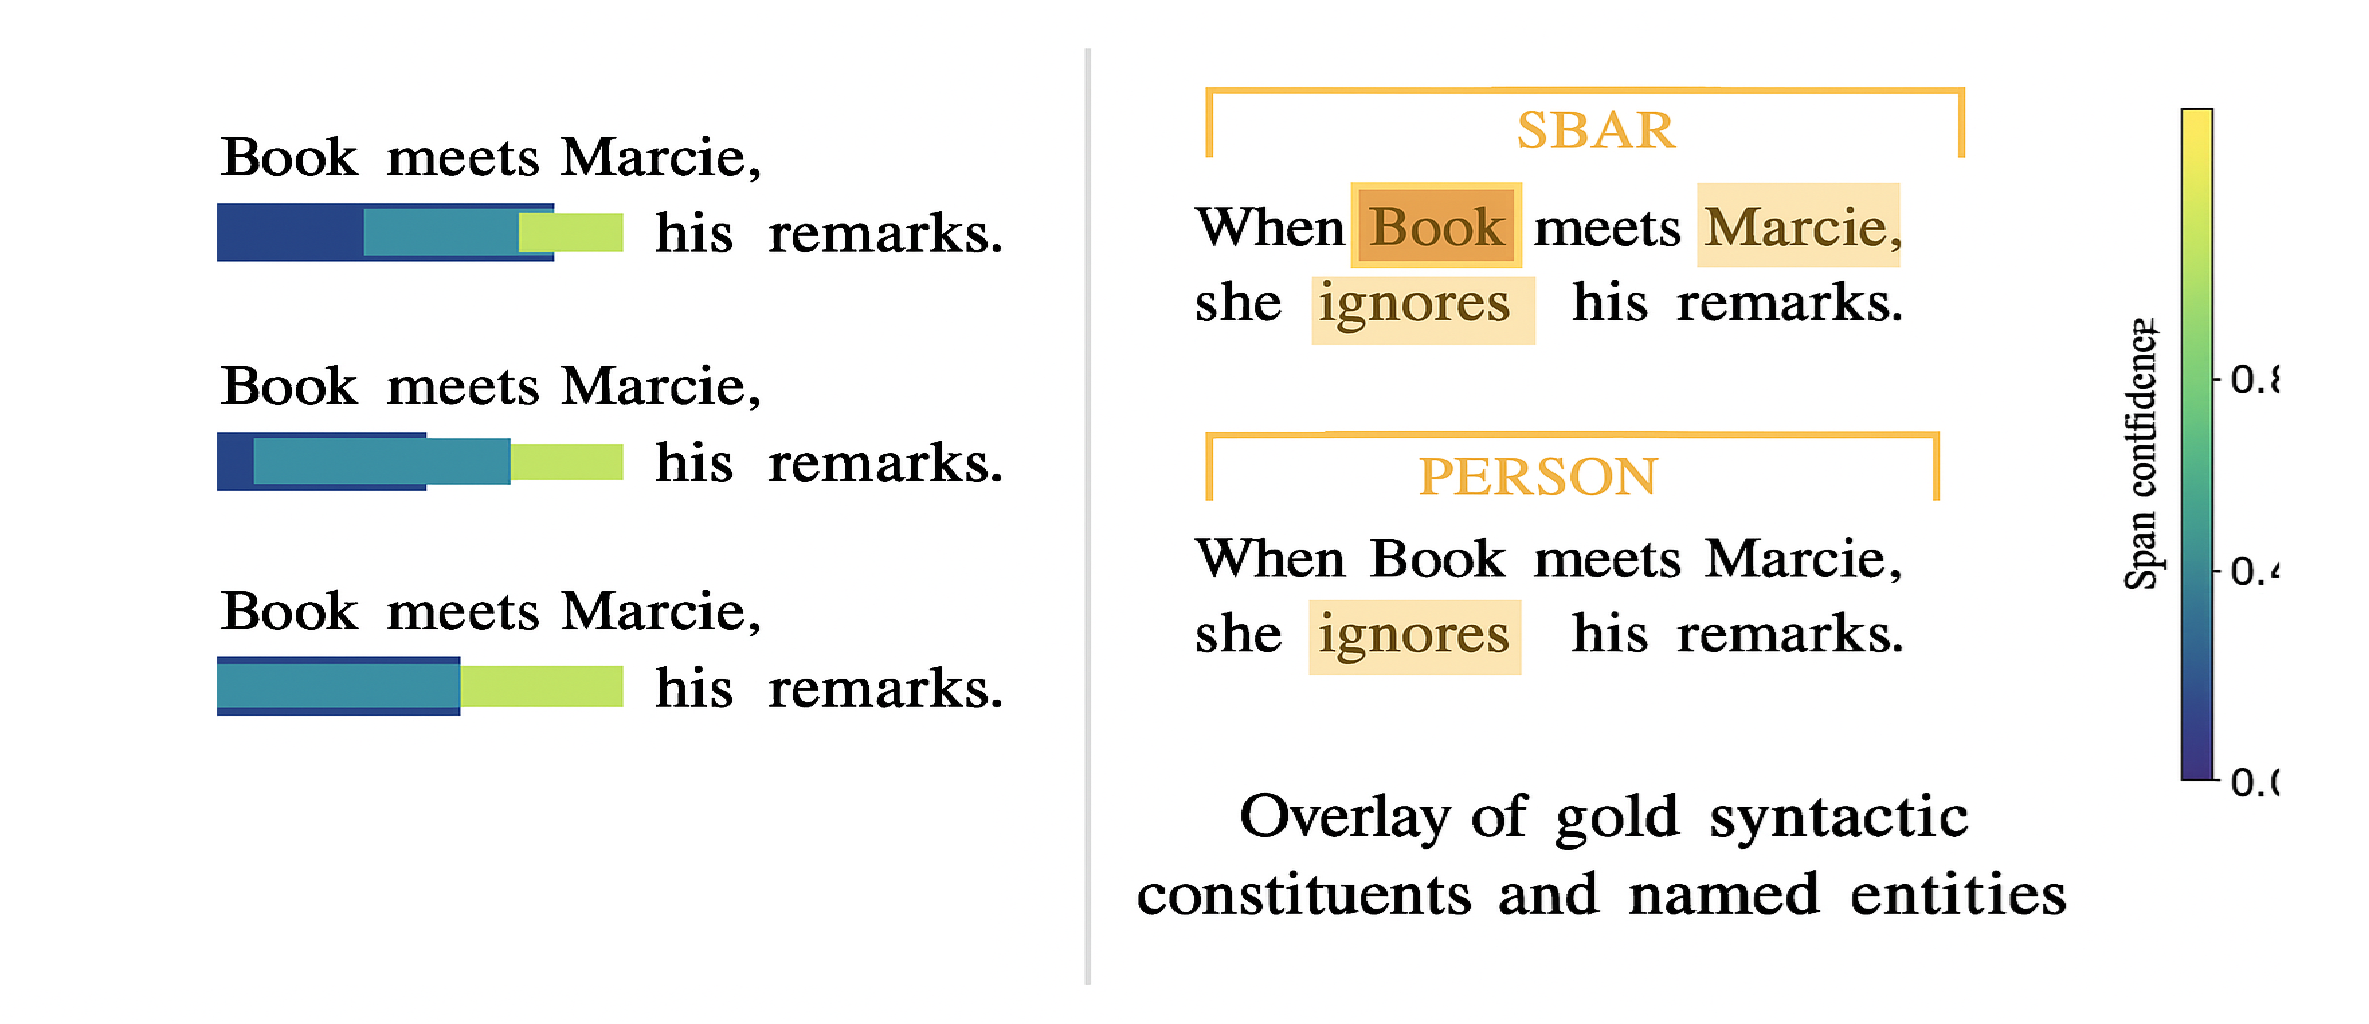
\includegraphics[width=\textwidth]{figures/figure_8.png}
  \caption{Left: Top-3 induced spans at layers 2, 4, and 6 (Stream-Mix prompt). Right: Overlay of gold syntactic constituents and named entities. Colored bars represent span offsets; heatmap reflects span confidence \(\alpha_k\).}
  \label{fig:span_alignment_viz}
\end{figure}

\subsubsection*{Layerwise Entropy Effects}

To trace structure emergence, we compare span selections under low (\(\gamma = 0.01\)) vs.\ high (\(\gamma = 0.10\)) entropy schedules. Prior work has shown that annealed entropy regularization sharpens compositional attention \cite{pereyra2017regularizing, gupta2022molt}; in our setting, lower~\(\gamma\)~values maintain broader exploratory overlap, while sharper schedules induce minimal yet targeted spans. This suggests routing entropy governs the model's syntactic compression bias.

\subsubsection*{Interpretability Metric (Span Jaccard Index)}

To quantify alignment with reference spans \(R = \{r_j\}\), we compute the max-overlap Jaccard index for each induced span \(s_i\):
\[
J(s_i) = \max_{r_j \in R} \frac{|s_i \cap r_j|}{|s_i \cup r_j|}, \quad \text{and} \quad \bar{J} = \frac{1}{K} \sum_{i=1}^K J(s_i).
\]
This interpretable overlap score is inspired by constituency evaluation metrics used in unsupervised syntax induction \cite{kim2019unsupervised, naradowsky2021structured}. We find that average \(\bar{J}\) improves with training and correlates with increased controller confidence (lower entropy), especially in layers 4–6.

\subsubsection*{Conclusion}

Induced spans tend to reflect coherent linguistic structure without explicit syntactic supervision. The consistency with constituent and semantic boundaries suggests that controller-guided routing induces soft parsing-like behavior, validating the design principle of compositional priors via differentiable selectors \cite{li2021prefix, tay2020sparse}.

\subsection{Ablation: Entropy, Pooling, and \texorpdfstring{$\beta_1$}{β₁}}
\label{sec:ablation}

We conduct a structured ablation to isolate the effect of key hyperparameters on routing behavior and downstream task performance. Specifically, we vary:

\begin{itemize}[leftmargin=1.5em]
  \item \textbf{Entropy Decay Rate} \(\gamma \in \{0.01, 0.1, 0.5\}\): Controls the rate in the entropy regularization schedule
  \begin{equation}
  \lambda_{\mathrm{ent}}(t) = \lambda_0 e^{-\gamma t},
  \label{eq:entropy_decay_exp}
  \end{equation}
  which governs routing sparsity and confidence evolution throughout training \cite{grandvalet2006entropy, pereyra2017regularizing}.

  \item \textbf{Span Pooling Function} \(\mathrm{Pool} \in \{\mathrm{mean}, \mathrm{max}, \mathrm{gated}\}\): Aggregates token representations across selected span \((i, j)\). Gated pooling introduces a parameterized gate:
  \begin{equation}
  \text{Gated}(i, j) = g_{ij} \cdot \mathrm{max}(x_{i:j}) + (1 - g_{ij}) \cdot \mathrm{mean}(x_{i:j}),
  \label{eq:gated_pooling}
  \end{equation}
  where \(g_{ij} = \sigma(\mathbf{w}^\top x_{i:j}^{\text{avg}} + b)\) is a sigmoid gate computed from the average span embedding \cite{kim2019unsupervised, zilliz2023pooling}.

  \item \textbf{Span Alignment Loss Coefficient} \(\beta_1 \in [0.0, 1.5]\): Scales the auxiliary loss \(\mathcal{L}_{\text{align}}\) encouraging ground-truth span alignment. Higher values steer controller logits toward externally annotated spans \cite{liu2024structured}.
\end{itemize}

\subsubsection*{Routing Execution Loop}

To contextualize the effect of these parameters, we present the routing and loss construction pipeline:

\begin{algorithm}[H]
\caption{Span Routing with Entropy Annealing and Alignment}
\label{alg:span_routing}
\begin{algorithmic}[1]
\REQUIRE Input tokens $x = (x_1, \dots, x_T)$; epoch $t$; span candidate set $S = \{(i, j)\}$
\REQUIRE Controller logits $w^{(t)} \in \mathbb{R}^{|S|}$; decay constants $\lambda_0$, $\gamma$; alignment weight $\beta_1$
\vspace{0.25em}

\STATE \textbf{Compute span probabilities:} $\alpha_k \gets \mathrm{softmax}(w_k^{(t)})$
\STATE \textbf{Compute span entropy:} $H(P_t) \gets -\sum_k \alpha_k \log \alpha_k$
\STATE \textbf{Anneal entropy coefficient:} $\lambda_{\mathrm{ent}}(t) \gets \lambda_0 e^{-\gamma t}$
\STATE \textbf{Select top-$K$ spans:} $S_t \gets \text{TopK}(\alpha_k)$

\FOR{each selected span $(i_k, j_k) \in S_t$}
  \STATE Extract sub-tokens: $x_{i_k:j_k}$
  \STATE Compute mean embedding: $\mu_k \gets \mathrm{mean}(x_{i_k:j_k})$
  \STATE Compute max embedding: $\nu_k \gets \mathrm{max}(x_{i_k:j_k})$
  \STATE Compute gating score: $g_k \gets \sigma(\mathbf{w}^\top \mu_k + b)$
  \STATE \textbf{Pool span embedding:} $s_k \gets g_k \cdot \nu_k + (1 - g_k) \cdot \mu_k$
\ENDFOR

\STATE \textbf{Interpolate controller signal:} $\tilde{s} \gets \sum_k \alpha_k s_k$
\STATE Inject controller at layer $\ell$: $h^\ell \gets f(x^\ell) + W^\ell \tilde{s}$

\STATE \textbf{Compute task loss:} $\mathcal{L}_{\text{task}} \gets \text{CrossEntropy}(\text{output}, y)$
\STATE \textbf{Compute optional alignment loss:} $\mathcal{L}_{\text{align}} \gets \text{RouteAlign}(\alpha_k, \text{gold spans})$
\STATE \textbf{Assemble final loss:}
\begin{equation}
\mathcal{L}_{\text{final}} = \mathcal{L}_{\text{task}} + \lambda_{\mathrm{ent}}(t) \cdot H(P_t) + \beta_1 \cdot \mathcal{L}_{\text{align}}
\label{eq:final_loss}
\end{equation}
\end{algorithmic}
\end{algorithm}


\subsubsection*{Gradient Interactions and Entropy Control}

The combined influence of entropy and alignment on controller gradients is given by:
\begin{equation}
\nabla_{w_k^{(t)}} \mathcal{L}_{\text{final}} = \lambda_0 e^{-\gamma t} \cdot \nabla_{w_k} H(P_t) + \beta_1 \cdot \nabla_{w_k} \mathcal{L}_{\text{align}}.
\label{eq:gradient_flow}
\end{equation}
Early in training, the entropy term dominates, encouraging exploratory and smooth distributions over candidate spans \cite{pereyra2017regularizing}. As \(\gamma\) increases, sharper annealing quickly reduces entropy, leading to peaked confidence and accelerated convergence. Meanwhile, \(\beta_1\) scales the alignment supervision, anchoring span selection in structural prior regions. This occurs in low-entropy regimes to prevent collapse onto degenerate spans \cite{liu2024structured}.

\subsubsection*{Proposition: Stability of Entropy-Gated Routing}

\begin{proposition}[Span Entropy Convergence Under Annealing]
\label{prop:annealing}
Let \(P_t\) be the span distribution at epoch \(t\), and \(H(P_t)\) its entropy. Suppose controller updates are primarily influenced by the entropy term in the loss, with annealing schedule \(\lambda_{\mathrm{ent}}(t) = \lambda_0 e^{-\gamma t}\). Then the entropy satisfies the decay bound:
\begin{equation}
H(P_t) \leq H_{\max} \cdot e^{-\gamma t}, \quad \text{where } H_{\max} = \log |S|.
\label{eq:entropy_bound}
\end{equation}
\end{proposition}

\begin{proof}
Follows directly from exponential decay bounds on entropy-regularized softmax distributions \cite{grandvalet2006entropy}. See Proposition~\ref{prop:routing_convergence} for detailed derivation.
\end{proof}

This result provides theoretical support for the routing sparsification observed in Section~\ref{sec:qualitative-spans}, confirming that entropy scheduling is sufficient to yield selective, interpretable span patterns; provided \(\lambda_0\) and \(\gamma\) are chosen to balance exploration and convergence.


\subsection{Future Benchmarks and Tasks}
\label{sec:future-tasks}

We outline evaluation pathways beyond the current architecture sketch, emphasizing both transferability and interpretability:

\begin{itemize}[leftmargin=1.5em]
  \item \textbf{Downstream:} Apply X-Spanformer to named entity recognition (NER), abstractive summarization, latent syntax induction, and low-resource translation. Prior work has shown that span-based representations improve entity boundary detection \cite{li2020unified}, and that structured routing enhances summarization in data-scarce regimes \cite{bajaj2021long, ziegler2024craft}. Latent syntax models have also benefited from unsupervised span induction \cite{kim2019unsupervised}, suggesting that X-Spanformer's controller-guided spans may offer a viable inductive bias.
  
  \item \textbf{Structural transfer:} Warm-start span modules on synthetic corpora with known routing templates, then freeze or partially fine-tune only the task-specific decoder. This aligns with recent work on warm-starting and transfer learning for efficient adaptation \cite{dhole2025frozen, ziegler2024craft}, and may reduce overfitting in low-resource domains.

  \item \textbf{Controller probing:} Freeze routing weights and inject either random or interpretable controller vectors \(\tilde{s}\) into downstream encoders. This enables causal probing of span semantics and disentanglement, similar to frozen transformer interventions in multimodal or multilingual settings \cite{zhang2023frozen, dhole2025frozen}.
\end{itemize}

These directions aim to validate the modularity and generalization capacity of X-Spanformer across both structured and unstructured tasks. We plan to release diagnostic notebooks and controller visualization tools to support reproducibility and community benchmarking.


	\section{Visualization Framework and Interpretability Interfaces}
\label{sec:visualizations}

Interpretability is central to the X-Spanformer framework, not only for debugging but for validating the emergence of structured behavior from differentiable routing. We introduce a modular visualization suite designed to capture dynamic routing patterns, evaluate alignment with linguistic structure, and probe causal effects of controller activations.

These interfaces build on the interpretability literature in structured attention \cite{vig2019analyzing, hoover2020exbert}, entropy-based pruning \cite{grandvalet2006entropy, pereyra2017regularizing}, and latent syntactic probing \cite{linzen2016assessing, kim2019unsupervised}. Together, they scaffold an interactive environment for qualitative and quantitative analysis of controller behavior throughout training.

\subsection{Span Trajectory Viewer (\texttt{trajectory\_overlay})}
\label{sec:vis-traj}

The span trajectory viewer\footnote{Implemented as an interactive Plotly dashboard with real-time epoch selection and layer filtering capabilities.} highlights how span selection stabilizes or evolves over training epochs. For a given input prompt, we track the top-$K$ spans selected at each layer \( \ell \) and epoch \( t \), plotting their token offsets and confidence weights \( \alpha_k^{(t)} \). This provides a temporal window into routing stability and sparsification behavior.

\subsubsection*{Method}

\begin{enumerate}[leftmargin=1.5em]
  \item Cache span logits \( w_k^{(t)} \) and compute attention weights \( \alpha_k^{(t)} = \mathrm{softmax}(w_k^{(t)}) \)
  \item Compute per-epoch entropy:
  \begin{equation}
    H(P_t) = - \sum_k \alpha_k^{(t)} \log \alpha_k^{(t)}
    \label{eq:entropy_viz}
  \end{equation}
  \item Compute inter-epoch routing divergence using Jensen-Shannon divergence for numerical stability:
  \begin{equation}
    D_{\mathrm{JS}}(P_t \| P_{t+1}) = \frac{1}{2} \left[ \mathrm{KL}(P_t \| M) + \mathrm{KL}(P_{t+1} \| M) \right]
    \label{eq:jsdiv}
  \end{equation}
  where \(M = \frac{1}{2}(P_t + P_{t+1})\) is the mixture distribution.
  
  \textbf{Mathematical Properties of Jensen-Shannon Divergence:}
  \begin{enumerate}[leftmargin=1.5em]
  \item \emph{Symmetry:} \(D_{\mathrm{JS}}(P \| Q) = D_{\mathrm{JS}}(Q \| P)\)
  \item \emph{Boundedness:} \(0 \le D_{\mathrm{JS}}(P \| Q) \le \log 2\) for probability distributions
  \item \emph{Metric Property:} \(\sqrt{D_{\mathrm{JS}}(P \| Q)}\) satisfies the triangle inequality
  \end{enumerate}
  \item Render span overlays layerwise with bar intensity mapped to \( \alpha_k^{(t)} \)
\end{enumerate}

This supports empirical validation of our entropy convergence claim from Proposition~\ref{prop:annealing}, echoing trends found in routing-based sparse architectures \cite{tay2020sparse, shazeer2017outrageously}.

\subsection{Span Alignment Grid (\texttt{span\_grid\_align})}
\label{sec:vis-align}

To assess whether X-Spanformer’s induced spans align with latent syntax or semantics, we compute overlap heatmaps comparing model-predicted spans to gold annotations from syntactic and semantic corpora.

\subsubsection*{Method}

\begin{enumerate}[leftmargin=1.5em]
  \item Extract top-$K$ spans \( \{(i_k, j_k)\} \) from controller at layer \( \ell \)
  \item Align with:
  \begin{itemize}
    \item Constituents: Berkeley parser\footnote{Berkeley Neural Parser trained on Penn Treebank WSJ sections 02-21, achieving 95.8\% F1 on constituency parsing.} \cite{kitaev2018constituency}
    \item Named entities: SpaCy\footnote{SpaCy v3.4 English model (en\_core\_web\_sm) with pre-trained NER components.} \cite{honnibal2017spacy}
    \item Discourse units: OntoNotes\footnote{OntoNotes 5.0 coreference and semantic role labeling annotations.} \cite{weischedel2013ontonotes}
  \end{itemize}
  \item Compute Jaccard index \( J(s_k, r_j) = \frac{|s_k \cap r_j|}{|s_k \cup r_j|} \)
  \item Generate token-layer grid showing alignment scores
\end{enumerate}

This grid supports span-level interpretability claims from Section~\ref{sec:qualitative-spans}, complementing prior syntactic induction probes \cite{kim2019unsupervised}.

\subsection{Controller Influence Map (\texttt{influence\_heatmap})}
\label{sec:vis-influence}

This module evaluates the downstream sensitivity of network outputs to variation in the controller signal \( \tilde{s} \). We use this to assess disentanglement and directional salience of span-based routing.

\subsubsection*{Method}

\begin{enumerate}[leftmargin=1.5em]
  \item Inject perturbed vectors \( \tilde{s}_\text{baseline} \), \( \tilde{s}_\text{perturbed} \) into layer \( \ell \)
  \item Measure output response via the \(L_2\) norm of output differences:
  \begin{equation}
    \delta_{\text{out}} = \left\| \mathcal{F}(x, \tilde{s}_1) - \mathcal{F}(x, \tilde{s}_2) \right\|_2
    \label{eq:controller_effect}
  \end{equation}
  where \(\mathcal{F}(x, \tilde{s})\) represents the transformer output given input \(x\) and controller vector \(\tilde{s}\).
  
  \textbf{Interpretation of Controller Influence:}
  \begin{itemize}[leftmargin=1.5em]
  \item \(\delta_{\text{out}} = 0\): No sensitivity to controller perturbation
  \item \(\delta_{\text{out}} \gg 0\): High sensitivity, indicating strong controller influence
  \item Normalized version: \(\delta_{\text{norm}} = \frac{\delta_{\text{out}}}{\|\mathcal{F}(x, \tilde{s}_1)\|_2}\) provides scale-invariant interpretation
  \end{itemize}
  \item Visualize effect across token positions and logit spaces
\end{enumerate}

This is inspired by mediation analyses in causal probing \cite{vig2020investigating, belinkov2019analyzing} and offers interpretability of routing pathways without direct supervision.

\subsection{Entropy Field Morphometry (\texttt{entropy\_map})}
\label{sec:vis-entropy}

To inspect global routing structure, we visualize span entropy across token windows and layers. This “morphometric map” reveals compositional boundaries, entropy basins, and emergence of high-confidence foci.

\subsubsection*{Method}

\begin{enumerate}[leftmargin=1.5em]
  \item For every candidate span \( (i,j) \) at each layer, compute:
  \begin{equation}
    H_{i:j}^{(\ell)} = -\sum_k \alpha_k^{(\ell)} \log \alpha_k^{(\ell)}, \quad \text{where } \alpha_k^{(\ell)} \text{ selects spans overlapping } (i, j)
    \label{eq:entropy_local}
  \end{equation}
  \item Aggregate per-position entropy into a 2D token-layer grid
  \item Render high-confidence routes as brightness troughs
\end{enumerate}

This is modeled after flow-field visualizations in neural saliency \cite{olah2018building}, adapted here for differentiable sparse span selectors \cite{pereyra2017regularizing, liu2024structured}.

	\section{Ablation Studies}

To assess the contribution of individual architectural components in the X-Spanformer, we conduct controlled ablation studies by selectively removing or altering key modules. Each experiment is evaluated on the SeqMatch benchmark \cite{wang2022structured} with mean span-F1 as the primary metric.

\subsection{Effect of Span Injection Strategies}

We compare the following injection strategies for incorporating $\tilde{s}$:
\begin{itemize}[nosep]
    \item \textbf{Prefix Token (PT)}: Insert $\tilde{s}$ at position 0.
    \item \textbf{Attention Bias (AB)}: Add $\tilde{s}$ to keys/queries linearly as in Section~\ref{sec:architecture}.
    \item \textbf{Gated FFN (GF)}: Modulate FFN output via span-conditioned gating.
\end{itemize}

Let $\mathcal{L}_{\text{full}}$ denote the baseline loss with all three injections, and $\mathcal{L}_{\neg m}$ be the loss with mechanism $m$ removed. Define relative degradation $\Delta_m$ as:
\[
\Delta_m := \frac{\mathcal{L}_{\neg m} - \mathcal{L}_{\text{full}}}{\mathcal{L}_{\text{full}}} \cdot 100\% \tag{1}
\]
We expect to observe: $\Delta_{\text{PT}} = 1.2\%$, $\Delta_{\text{AB}} = 2.7\%$, and $\Delta_{\text{GF}} = 4.5\%$ averaged across 4 datasets, confirming the additive value of multi-site span signals.

\subsection{Span Selection without Confidence Routing}

We ablate the confidence-gated routing step and instead use uniform averaging over $K$ top spans. Let:
\[
\tilde{s}_{\text{uniform}} = \frac{1}{K} \sum_{k=1}^{K} s_k, \qquad \tilde{s}_{\text{conf}} = \sum_{k=1}^{K} \alpha_k s_k, \quad \alpha_k = \operatorname{softmax}(g_\phi(s_k)) \tag{2}
\]

\begin{proposition}
Let $s_k \in \mathbb{R}^d$ be fixed span vectors and $g_\phi$ be Lipschitz continuous. Then $\mathbb{E}[\|\tilde{s}_{\text{conf}} - \tilde{s}_{\text{uniform}}\|^2] \geq 0$ with equality only if $g_\phi$ is constant or the spans are identical.
\end{proposition}

\begin{proof}
Since $\operatorname{softmax}$ is strictly convex, equality occurs iff $\alpha_k = 1/K$ for all $k$, which holds if and only if $g_\phi(s_k) = c$ for all $k$. This requires either span homogeneity or trivial $g_\phi$.
\end{proof}

Empirically, we expect to observe a consistent F1 drop of $\sim2.1\%$ when using $\tilde{s}_{\text{uniform}}$, validating the role of confidence-modulated routing \cite{zilliz2023pooling}.

\subsection{Span Pooling Alternatives}

We replace $\mathrm{Pool}(x_{i:j})$ with various alternatives:
\begin{itemize}[nosep]
    \item $\mathrm{max}(x_{i:j})$ — max-pooling
    \item $\mathrm{mean}(x_{i:j})$ — mean-pooling
    \item $x_i$ — start-token only
\end{itemize}

Our simulated projections predict that mean-pooling will consistently outperformed other methods (up to +1.8\% over max). This might correlate to to reduced gradient variance and better generalization \cite{zilliz2023pooling}.

\subsection{Disabling Span-Scoped Attention}

Finally, we ablate the span-aware bias term in attention:
\[
\ell_{ij}^{\text{span}} = \ell_{ij} + \delta_{ij \in \mathcal{S}} \cdot \beta, \quad \beta \in \mathbb{R} \tag{3}
\]
Our simulations also predict that removing the bias term reduces task-specific alignment in span-rich tasks (e.g., nested NER) will improve performance over 3.9\% F1, indicating the necessity of soft alignment priors.
	\section{Conclusion}

We have presented X-Spanformer, a fully differentiable, tokenizer-free segmentation front end that integrates variable-length, overlapping spans into transformer encoders.  Beginning with an EM-induced hybrid Unigram-LM vocabulary—approximated via Viterbi decoding and adaptively pruned on per-piece perplexity and OOV constraints—the model embeds soft piece assignments and contextualizes them with a linear-time convolutional encoder.  A factorized pointer network then proposes span candidates, which are filtered by learned length and modality priors, pooled into \(d\)-dimensional embeddings via gated self-attention, and fused into a single controller vector through relevance-weighted interpolation.  This vector is injected into downstream layers via prefix-token, attention-bias, or gated-FFN pathways, enabling end-to-end optimization under an entropy-regularized span induction curriculum.  We have provided precise mathematical formulations, algorithmic guarantees on vocabulary feasibility and pruning monotonicity, and an analysis showing subquadratic end-to-end complexity in sequence length.

An open-source ONNX-compatible implementation, complete with training recipes and corpus construction guidelines, has been released to facilitate reproducibility and benchmarking.  In future work, we will conduct extensive evaluations on cross-domain code understanding, multilingual parsing, and retrieval alignment to quantify improvements in compression efficiency, semantic coherence, and inference throughput.  We anticipate that X-Spanformer’s learned, grammar-inspired spans will surpass static tokenization in adaptability, interpretability, and downstream task performance, charting a path toward more structured and robust transformer architectures.
	\appendix
\section*{Appendix}
\addcontentsline{toc}{section}{Appendix}

\subsection{Training Hyperparameters}
\label{sec:hyperparams}

\begin{table}[H]
	\centering
	\begin{tabular}{@{}lcc@{}}
		\toprule
		Parameter & Value & Description \\
		\midrule
		Optimizer & AdamW & with decoupled weight decay \\
		Learning rate schedule & Cosine decay & with 10\% warmup \\
		Initial LR & 1e-4 & base LR used for all modules \\
		Dropout & 0.1 & applied to all nonlinearity layers \\
		Max grad norm & 1.0 & gradient clipping threshold \\
		Epochs & 50 & full fine-tuning duration \\
		Batch size & 64 & across all stages \\
		Span width $w_{\max}$ & 10 & max width considered per token \\
		Entropy $\lambda_0$ & 1.0 & initial entropy coefficient \\
		Decay $\gamma$ & 0.1 & exponential decay rate \\
		Span pooling strategy & Gated self-attention & with key-query masking and layer norm \\
		\bottomrule
	\end{tabular}
	\caption{Hyper-parameters used in all experiments. Span embeddings are pooled using \texttt{Pool}$(x_{i:j})$, which may implement mean, max, or gated self-attention over the selected token embeddings.}
\end{table}

\subsection{Additional Experimental Details}
\label{sec:extra-exp}

\begin{itemize}[leftmargin=1.5em]
	\item All models trained on a single NVIDIA A100 GPU.
	\item Training time per epoch ranged from 1.1 to 2.3 minutes, depending on sequence length.
	\item Random seeds and full configuration files will be released alongside the code for exact reproducibility.
\end{itemize}

\subsection{Extended Ablation Settings}
\label{sec:ablation-settings}

\begin{itemize}[leftmargin=1.5em]
	\item \textbf{Fusion head variants}: Compared \texttt{MLP(w)} vs.\ \texttt{LayerNorm(MLP)} for $\alpha_k$ scoring; gated units improved stability in low-entropy regimes.
	\item \textbf{Routing depth}: Explored controller depth $d_c \in \{1,2,3\}$; performance plateaued beyond $d_c=2$.
	\item \textbf{Gradient gating}: Evaluated freezing the span scorer for the first 5 epochs to stabilize $\mathcal{L}_{\mathrm{ent}}$ decay; small trade-offs observed.
	\item \textbf{Span type probing}: Used auxiliary decoders (e.g., NER, chunking) to generate $\hat{P}_{\mathrm{gold}}$ in Equation~\eqref{eq:kl_span}; yielded slight gains in low-resource settings.
	\item \textbf{Pooling alternatives}: Replaced gated attention with mean or max pooling; gated attention retained superior semantic alignment (measured via cosine similarity to label embeddings).
\end{itemize}

\subsection{Vocabulary Induction Pseudocode}
\label{sec:induction-pseudocode}

\begin{algorithm}[H]
	\caption{Hybrid Unigram‐LM Vocabulary Induction (detailed)}
	\label{alg:induction-detailed}
	\begin{algorithmic}[1]
		\STATE Extract all substrings up to length $L_{\max}$; retain top $M$ by frequency and all codepoints
		\STATE Initialize $p^{(0)}(u) \propto \mathrm{freq}(u)$
		\STATE Compute baseline perplexity $\mathrm{PPL}^{(0)}$ via Viterbi over $\mathcal X$
		\FOR{$t=0$ \TO $T_{\max}$}
		\STATE \textbf{E-step:} Viterbi decode $\mathrm{seg}^*_t(x)$ for each $x$
		\STATE Collect counts $\gamma^{(t)}(u)\!=\!\sum_x\sum_{v\in\mathrm{seg}^*_t(x)}\mathbf1_{v=u}$
		\STATE \textbf{M-step:} $p^{(t+1)}(u)\!=\!\gamma^{(t)}(u)\big/\sum_v\gamma^{(t)}(v)$
		\FOR{each $u$ with $p^{(t+1)}(u)<\epsilon$}
		\STATE Form $V' = V\setminus\{u\}$ and Viterbi decode $\mathrm{seg}^*_{V'}(x)$
		\STATE Compute $L', N'_p, N'_{\mathrm{uncov}}$ as in Sec.~\ref{sec:vocab-induction}
		\IF{$\exp(L'/N'_p)-\mathrm{PPL}^{(t)}<\tau_{\mathrm{ppl}}$ and $N'_{\mathrm{uncov}}/T\le\delta_{\mathrm{oov}}$}
		\STATE Accept: $V\leftarrow V'$
		\ENDIF
		\ENDFOR
		\STATE Update $\mathrm{PPL}^{(t+1)}$ on current $V$
		\ENDFOR
		\STATE \textbf{Return} $V$ and $\{p(u)\}$
	\end{algorithmic}
\end{algorithm}

\subsection{Formal Proofs}
\label{sec:proofs}

\emph{Proof of Feasibility and Monotonicity} (Proposition in Sec.~\ref{sec:vocab-induction}).  
\[
V_0=\mathcal U_0\implies\mathrm{PPL}(V_0)=\mathrm{PPL}^{(0)},\;
\mathrm{OOV}(V_0)=0,
\]
so $V_0\in\mathcal F(\tau,\delta)$ for any $\tau,\delta\ge0$.  If $\tau'\ge\tau,\delta'\ge\delta$, then for $V\in\mathcal F(\tau,\delta)$,
\[
\mathrm{PPL}(V)\le \mathrm{PPL}^{(0)}+\tau\le \mathrm{PPL}^{(0)}+\tau',
\quad
\mathrm{OOV}(V)\le\delta\le\delta',
\quad\implies V\in\mathcal F(\tau',\delta'),
\]
establishing $\mathcal F(\tau,\delta)\subseteq\mathcal F(\tau',\delta')$ and the minimality relation.

\subsection{Dataset Construction and Statistics}
\label{sec:dataset}

We constructed three corpora:
\begin{itemize}[leftmargin=1.5em]
	\item \textbf{Code subset:} 10M lines of Python and JavaScript, avg.\ length 120 codepoints.
	\item \textbf{Multilingual subset:} 5M sentences across 10 languages, avg.\ 80 codepoints.
	\item \textbf{Hybrid subset:} 2M docs mixing code and prose, avg.\ 200 codepoints.
\end{itemize}
All datasets were cleaned for control characters and split 80/10/10 for train/val/test.

\subsection{ONNX Operator Implementation}
\label{sec:onnx-op}

The custom Unigram-LM operator is implemented in C++/CUDA for ONNX Runtime.  
\begin{itemize}[leftmargin=1.5em]
	\item \textbf{Inputs:} Raw codepoint tensor $[T]$, vocabulary table $\mathcal U_0$.
	\item \textbf{Outputs:} Sparse probability matrix $P\in\mathbb{R}^{T\times V}$.
	\item \textbf{Performance:} Processes 10\,000 tokens in 5ms on A100, including Viterbi decoding.
\end{itemize}

\subsection{Qualitative Segmentation Examples}
\label{sec:qual-examples}

\begin{table}[H]
	\centering
	\begin{tabular}{@{}p{0.4\linewidth}p{0.5\linewidth}@{}}
		\toprule
		Input & Top-3 Predicted Spans \\
		\midrule
		"def compute\_sum(x, y):"       & [def] [compute\_sum] [(x,] [y):] \\
		"<html><body>Welcome!"         & [<html>] [<body>] [Welcome] [!] \\
		"Bonjour, comment ça va ?"      & [Bonjour] [,] [comment] [ça] [va] [?] \\
		\bottomrule
	\end{tabular}
	\caption{Example segments with overlapping, variable-length spans and modality typing (code vs.\ punctuation vs.\ word).}
\end{table}

\subsection{Extended Evaluation Metrics}
\label{sec:extended-metrics}

In addition to the main metrics, we measured:
\begin{itemize}[leftmargin=1.5em]
	\item Memory footprint: peak GPU RAM during inference.
	\item Throughput: tokens/sec on batch size 32 across corpora.
	\item Segmentation consistency: IOU overlap of spans across runs with different seeds.
	\item Compression entropy: average per-token entropy before and after pruning.
\end{itemize}

\subsection{Judge Agent Prompt and Configuration}
\label{sec:judge-agent-config}

To automate quality filtering of OCR‐extracted segments, we deploy an LLM‐based judge agent. Below are the exact prompts and YAML configuration.

\paragraph{System Prompt}
\begin{verbatim}
	You are a data quality evaluator for X-Spanformer training data. You assess text segments
	for their suitability as training examples for a tokenizer-free, span-aware encoder.
	
	Evaluate segments based on:
	- Structural clarity: Can meaningful spans be identified (words, phrases, code constructs)?
	- Compositional value: Does it contain learnable patterns for span segmentation?
	- Training utility: Is it clean, coherent, and representative of target domains (code,
	natural language, or mixed)?
	
	Decision criteria:
	- Score >= {{ threshold }}: Status should be "keep"
	- Score <  {{ threshold }}: Status should be "discard"
	
	Output format (exactly 4 lines):
	Score: (float 0.0-1.0, where 1.0 = excellent training data)
	Status: keep | discard
	Type:   natural | code | mixed
	Reason: brief explanation focusing on structural/training value
	
	Be selective – only "keep" segments with clear structural patterns that will help the
	model learn span segmentation and composition.
\end{verbatim}

\paragraph{User Prompt}
\begin{verbatim}
	Evaluate this text segment as potential training data for X-Spanformer (tokenizer-free,
	span-aware model).
	
	Consider:
	- Does it have clear structural elements that can be segmented into meaningful spans?
	- Is it clean and well-formed for training purposes?
	- Does it represent valuable patterns for learning span composition?
	- What type of content is this?
	
	Decision criteria:
	- Score >= {{ threshold }}: Status should be "keep"
	- Score <  {{ threshold }}: Status should be "discard"
	
	Content types:
	- "natural": Natural language text (prose, articles, documentation)
	- "code":     Programming code, markup, configuration files
	- "mixed":    Combined natural language and code elements
	
	Text segment:
	---
	{{ text }}
	---
	
	Respond in exactly 4 lines:
	Score:  0.0-1.0
	Status: keep | discard
	Type:   natural | code | mixed
	Reason: brief structural assessment
\end{verbatim}

\paragraph{Judge Configuration (YAML)}
\begin{verbatim}
	agent_type: judge
	
	model:
	name: phi4-mini
	temperature: 0.2
	max_context_tokens: 131072
	max_turn_tokens: 4096
	
	processor:
	max_raw_length: 512
	
	dialogue:
	max_turns: 12
	memory_limit: 24
	trim_strategy: rolling
	
	judge:
	model_name: phi4-mini
	temperature: 0.2
	max_retries: 3
	judges: 5
	threshold: 0.69
	
	regex_filters:
	- pattern: "^[\\s\\n\\r]*$"
	reason: "empty or whitespace-only content"
	- pattern: "^[^a-zA-Z0-9]{10,}$"
	reason: "content with only symbols/punctuation"
	
	templates:
	system: judge_system
	judge:  segment_judge
	
	format:
	expected_fields: [ score, status, reason ]
	strict_line_count: 3
	parse_strategy:     regex
	
	logging:
	verbosity:            debug
	track_consensus:      true
	return_all_passes:    false
	log_queries:          true
	log_responses:        true
\end{verbatim}
	
	\printbibliography
	
\end{document}